% Load the base class
\documentclass[minted, draw]{../tex/hebdomon}
\usepackage{svg}
\usepackage{biblatex}[backend=biber, style=ieee, sorting=none]
\addbibresource{references.bib}
\usepackage[export]{adjustbox} % Per aggiungere bordi
\begin{document}



\publishers{
  \begin{tabular}[!b]{rl}
  \textbf{Student Name} & Achille Cannavale \\[3pt]
  \textbf{Student Number} & xxxxx \\[3pt]
  \textbf{Module Name} & xxxxx
  \end{tabular}\\[20pt]
  }

\begin{titlepage}
    \centering
    {\scshape\LARGE Università degli Studi di Cassino e del Lazio Meridionale\par}
    {\Large \textbf{Dipartimento di Ingegneria Elettrica e dell'Informazione} \par}
    \vspace*{2cm}
	
\includegraphics[width=4cm]{figures/logo.png}\par\vspace{1cm}

    %\vspace*{2cm}

    \vspace{1cm}
    {\Large \textbf{Corso di Laurea Magistrale in Ingegneria Informatica} \par}

    \vspace{1cm}
    {\Huge\bfseries Segmentazione del seno in immagini MRI\par}
    \vspace{1cm}

    \vfill

    \begin{flushleft}
    \textbf{Studente}: Achille Cannavale \\
	\textbf{Matricola}: 58721 \\
    \textbf{Relatore}: Alessandro Bria \\
    \textbf{Correlatore}: Marco Cantone \\
    \end{flushleft}

    \vspace{1.5cm}

    \begin{center}
        A.A 2024/2025
    \end{center}

\end{titlepage}

\dominitoc
\tableofcontents
\newpage



\Chapter{Introduzione}
\Section{Contesto}

La segmentazione di strutture anatomiche in immagini mediche 3D rappresenta un task importante nell’ambito clinico e diagnostico. In particolare la segmentazione del seno da immagini MRI (Magnetic Resonance Imaging) 3D è un task complesso, ma essenziale per applicazioni come la pianificazione di interventi chirugici o l’analisi di anomalie tessutali.

In passato, la segmentazione del seno in immagini MRI 3D veniva effettuata principalmente con \textbf{metodi classici}, spesso semi-automatici o manuali, basati su:

\begin{itemize}
	\item \hlight{Approcci a soglia} (thresholding) e \hlight{region-growing}, che sfruttavano differenze di intensità tra tessuti ma richiedevano regolazioni manuali e fallivano in presenza di rumore o basso contrasto.
	\item \hlight{Deformable models} (es.: Active Contours) e \hlight{algoritmi a clustering} (es.: k-means), sensibili all’inizializzazione e poco robusti alla variabilità anatomica.
	\item Metodi \hlight{atlas-based}, che allineavano immagini a template pre-annotati, limitati però dalla diversità inter-paziente.
\end{itemize}

Con l’avvento del \textbf{deep learning}, in particolar modo delle \textbf{reti convoluzionali} e di architetture come \hlight{U-Net 3D} \cite{chen2021transunet}, la segmentazione del seno ha raggiunto livelli di accuratezza più alti rispetto al passato. 




\Section{Attività di Tirocinio e obiettivi}

L’attività si è inserita nel contesto di un progetto di ricerca mirato allo sviluppo e alla valutazione di modelli di segmentazione automatica per immagini in MRI del seno, con l’obiettivo di migliorare la diagnosi precoce e la pianificazione terapeutica.

L’obiettivo principale del tirocinio è stato quello di sperimentare e ottimizzare pipeline basate su \textbf{deep learning} per la segmentazione semantica tridimensionale, utilizzando framework open-source moderni come \textbf{MONAI} (Medical Open Network for AI) \cite{cardoso2022monai} e \textbf{PyTorch}.

Le principali attività svolte durante il tirocinio sono state:
\begin{itemize}
    \item \textbf{Pre-processing} dei dati in formato DICOM, con conversione in formato leggibile da MONAI e normalizzazione delle immagini.
    \item Composizione e validazione di un dataset bilanciato, con partizionamento in training, validation e test set.
    \item Studio e implementazione di modelli di segmentazione basati su architetture tra cui \textbf{UNet} e \textbf{AttentionUNet}.
    \item Configurazione degli esperimenti, \textbf{tuning degli iperparametri} e addestramento dei modelli in ambiente GPU.
    \item Valutazione delle prestazioni mediante metriche standard come Dice Score
\end{itemize}

Durante il tirocinio sono state inoltre affrontate e risolte diverse problematiche tecniche legate alla gestione dei metadati DICOM, alla compatibilità tra i formati di input, e alla gestione efficiente della memoria in fase di training. L'intero lavoro è stato documentato e riproducibile mediante script \textbf{Python} e configurazioni \textbf{YAML}.


	
\Section{Strumenti Utilizzati}
Durante il tirocinio sono stati impiegati diversi strumenti software e librerie  fondamentali per la gestione, il pre-processing e l'elaborazione di immagini medicali, nonché per lo sviluppo e il training di modelli di deep learning.
\begin{itemize}
	\item  Il linguaggio principale di lavoro è stato \textbf{Python}, scelto per la sua flessibilità e per l'ampio ecosistema di librerie scientifiche.
	\item Per la manipolazione delle immagini DICOM è stata utilizzata la libreria \textbf{MONAI} (Medical Open Network for AI), un framework open-source basato su PyTorch e progettato specificamente per applicazioni di imaging medicale. MONAI ha permesso di gestire agevolmente il caricamento dei dati, le trasformazioni e la normalizzazione delle immagini, grazie a un sistema modulare di trasformazioni componibili.
	\item Il framework di deep learning impiegato è stato \textbf{PyTorch}, scelto per la sua semplicità d'uso, il supporto attivo della community e le sue prestazioni elevate, specialmente in combinazione con l'accelerazione GPU fornita da CUDA.
	\item Lo sviluppo del codice è stato realizzato su una macchina Linux, con accesso remoto e con l'ausilio dell'editor \textbf{Visual Studio Code}.
\end{itemize}


\Subsection{Connessione in SSH e GPU}

Durante il tirocinio, ho avuto accesso alla potenza di calcolo delle \textbf{GPU universitarie}, dedicate a progetti di ricerca in deep learning. Per sfruttare queste risorse, ho utilizzato il protocollo \textbf{SSH} (Secure Shell) \ref{fig:gpu_info} per connettermi in remoto ai server e gestire l’esecuzione dei miei esperimenti.

Il sistema era dotato di 4 GPU NVIDIA (modello Tesla V100 o A100, a seconda della disponibilità), condivise tra diversi utenti del dipartimento. Per evitare conflitti nell’allocazione delle risorse, è stato necessario prenotare in anticipo le GPU tramite un sistema di schedulazione interno, basato su code di priorità.

Nel dettaglio, il nodo su cui ho lavorato disponeva delle seguenti GPU:
\begin{itemize}
\item \textbf{3x NVIDIA Tesla V100-PCIE-16GB}, GPU ad alte prestazioni con 16 GB di memoria, molto diffuse in ambito scientifico per il training di deep neural networks.
\item \textbf{1x NVIDIA A100 80GB PCIe}, una delle GPU più potenti attualmente disponibili per il calcolo scientifico, con ben 80 GB di memoria dedicata. 
\end{itemize}

Le informazioni mostrate da \texttt{nvidia-smi} includevano anche temperatura, consumo energetico, utilizzo della memoria e livello di attività di ciascuna GPU. 

Questa infrastruttura ha permesso di testare i miei modelli su dataset di grandi dimensioni con tempi di addestramento molto più rapidi rispetto all’uso di una macchina locale.

\begin{figure}[H] 
  	\centering 
 	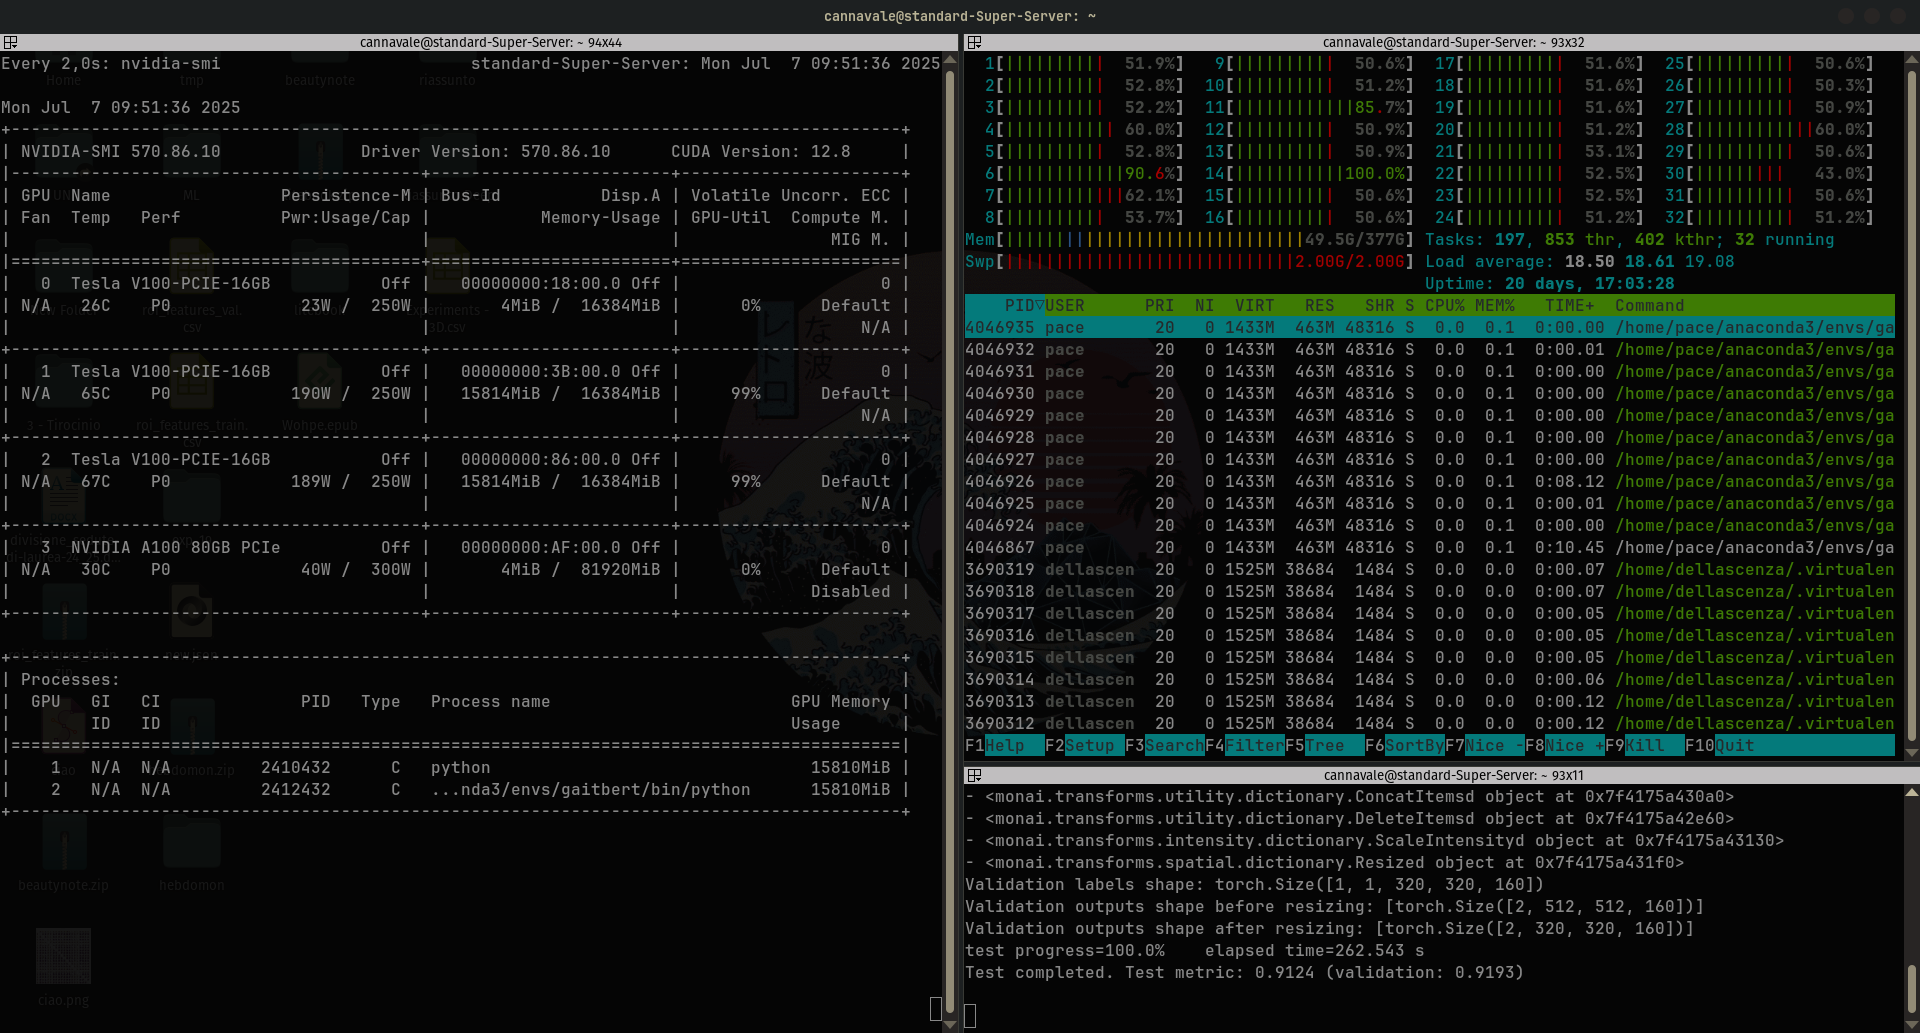
\includegraphics[width=\textwidth]{images/2025-07-07-09-52-55.png} 
	 \caption{Esempio di output del comando \texttt{nvidia-smi} per monitorare le GPU disponibili.}
	 \label{fig:gpu_info}
 \end{figure} 
\Chapter{Background e Stato dell'Arte}


La segmentazione semantica di immagini mediche rappresenta una delle sfide più importanti nel campo della diagnostica. Questo compito, che consiste nel delineare con precisione strutture anatomiche o aree patologiche all’interno di immagini biomediche, ha un impatto diretto su applicazioni cliniche cruciali come la pianificazione chirurgica e il monitoraggio terapeutico. Nel contesto specifico della mammella, la segmentazione da immagini MRI 3D presenta peculiarità che la rendono particolarmente complessa, tra cui l’elevata variabilità anatomica tra pazienti, la presenza di artefatti tipici delle risonanze magnetiche e la necessità di bilanciare accuratezza e tempi di elaborazione quando si lavora con volumi tridimensionali ad alta risoluzione.

\Section{L’Evoluzione delle Tecniche di Segmentazione}

Prima dell’avvento del deep learning, la segmentazione di immagini mediche si basava principalmente su approcci tradizionali che, pur rappresentando soluzioni pionieristiche per l’epoca, presentavano limiti significativi. Tecniche come il \textbf{thresholding} e il \textbf{region-growing}, ad esempio, erano ampiamente utilizzate per la loro semplicità concettuale, ma risultavano estremamente sensibili alla qualità dell’immagine, fallendo spesso in presenza di rumore o basso contrasto tra i tessuti. Allo stesso modo, i \textbf{deformable models}, che cercavano di adattare contorni attivi alle strutture anatomiche, richiedevano un’inizializzazione manuale e faticavano a gestire la complessa morfologia della ghiandola mammaria.

Con l’introduzione delle reti \hlight{neurali convoluzionali} (CNN), il panorama della segmentazione medica è cambiato radicalmente. L’architettura \hlight{U-Net}, proposta nel 2015 da \textbf{Ronneberger et al.,} ha rappresentato una svolta grazie alla sua struttura \textbf{encoder-decoder} e alle \textbf{skip connections}, che permettono di combinare informazioni a diversi livelli di risoluzione, preservando i dettagli spaziali fondamentali per una segmentazione precisa. Successivamente, la comunità scientifica ha sviluppato varianti sempre più avanzate, come la \textbf{V-Net}, ottimizzata per dati volumetrici, e il framework \textbf{nnU-Net}, in grado di adattarsi automaticamente alle caratteristiche di diversi dataset medici.

Negli ultimi anni, l’attenzione si è spostata verso i \hlight{Transformers}, modelli nati nell’ambito del \textbf{Natural Language Processing} e poi adattati con successo all’analisi di immagini. Architetture come \hlight{TransUNet} e \hlight{Swin UNETR} combinano la capacità delle CNN di estrarre features locali con il potere dei Transformers di modellare relazioni globali, offrendo prestazioni superiori in molti task di segmentazione. Tuttavia, questi modelli richiedono risorse computazionali elevate e grandi quantità di dati annotati, il che ne limenta ancora l’applicabilità in alcuni contesti clinici.


\Section{Architettura U-Net per la Segmentazione di Immagini Mediche}

Tra le architetture più utilizzate nel campo della segmentazione semantica applicata all’imaging biomedico, la \textbf{U-Net} occupa senza dubbio un ruolo di primo piano. Introdotta da Ronneberger et al. nel 2015, questa rete è stata progettata appositamente per segmentare immagini mediche anche in condizioni di disponibilità limitata di dati annotati, un aspetto ricorrente nei contesti clinici reali. Il successo della U-Net è dovuto non solo alla sua efficacia, ma anche alla sua semplicità architetturale, che la rende estremamente versatile e facilmente adattabile a diverse tipologie di dati, tra cui immagini 2D, 3D o multi-canale.

L'architettura della U-Net si sviluppa secondo una struttura simmetrica a forma di U \ref{fig:Schema concettuale dell'architettura U-Net}, composta da due fasi principali: un percorso di contrazione, o encoder, e un percorso di espansione, o decoder. La fase di contrazione ha il compito di estrarre rappresentazioni sempre più astratte e semantiche dell’immagine in input, riducendone progressivamente la risoluzione attraverso convoluzioni e operazioni di pooling. Al contrario, la fase di espansione mira a ricostruire l’informazione spaziale originaria, riportando l’output alla dimensione dell’immagine di partenza mediante operazioni di upsampling e convoluzioni.

\begin{figure}[H]
  	\centering 
 	\includegraphics[width=.6\textwidth]{figures/U-Net-architecture.png} 
	 \caption{Schema concettuale dell'architettura U-Net.}
	 \label{fig:Schema concettuale dell'architettura U-Net}
	\end{figure} 

Una caratteristica distintiva della U-Net rispetto ad altre reti di segmentazione è la presenza delle cosiddette \textit{skip connections}. Questi collegamenti diretti tra i livelli corrispondenti dell’encoder e del decoder permettono di trasportare le informazioni a bassa astrazione, spesso perse durante il downsampling, direttamente nei livelli di ricostruzione. In questo modo, la rete riesce a combinare efficacemente il contesto globale dell’immagine con i dettagli locali, migliorando significativamente la precisione dei bordi e la definizione delle strutture segmentate.

Dal punto di vista pratico, la U-Net prende in input un’immagine e produce come output una maschera segmentata, in cui ogni pixel (o voxel nel caso 3D) è classificato in una determinata categoria. Questo rende la rete particolarmente adatta per compiti dove è richiesta una segmentazione voxel-wise, come nel caso dell’identificazione di tessuti, lesioni o strutture anatomiche specifiche.

Nel progetto descritto in questa tesi, la U-Net è stata adottata come architettura di base per la segmentazione automatica del seno e del tessuto fibroghiandolare in immagini MRI. Questo approccio è ispirato anche al lavoro recente di Lew et al. (2024), in cui due reti U-Net sono state combinate in cascata per segmentare prima il seno intero e successivamente il tessuto interno, comprendente FGT e vasi sanguigni. In tal senso, la U-Net si è dimostrata una scelta solida, grazie alla sua capacità di generalizzare anche su strutture anatomiche complesse, pur mantenendo una buona efficienza computazionale.

Nonostante la sua efficacia, la U-Net presenta alcune limitazioni. In presenza di rumore, artefatti o grandi squilibri tra le classi, la rete può mostrare difficoltà, ad esempio nel riconoscere strutture piccole o nel distinguere tessuti contigui con caratteristiche simili. Per superare tali difficoltà, sono state sviluppate diverse estensioni e varianti dell’architettura originale, come l’U-Net++ con connessioni più profonde, le U-Net con meccanismi di attention, o le versioni 3D per dati volumetrici. Tuttavia, anche nella sua forma standard, la U-Net continua a rappresentare un punto di partenza solido e affidabile per molte applicazioni di segmentazione in ambito medico.




\Section{Strumenti e Dataset Moderni}
Oggi, lo sviluppo di pipeline per la segmentazione medica si avvale di strumenti sempre più sofisticati. Tra questi, il framework MONAI (Medical Open Network for AI) si è affermato come uno standard de facto, grazie alla sua vasta raccolta di trasformazioni specifiche per immagini mediche, modelli predefiniti e metriche di valutazione. Basato su PyTorch, MONAI semplifica notevolmente la gestione di dati complessi come quelli DICOM e supporta l’implementazione di workflow riproducibili, essenziali per la ricerca in ambito medico.

Per quanto riguarda i dataset, il Duke-Breast-Cancer-MRI, disponibile su The Cancer Imaging Archive (TCIA), rappresenta una risorsa preziosa per lo studio della segmentazione mammaria. Questo dataset include volumi MRI multiparametrici annotati manualmente da radiologi esperti, catturando tutta la complessità anatomica e le sfide tipiche delle immagini reali, come la presenza di lesioni e la variabilità nella densità del tessuto.


\Section{Stato dell'Arte nella Segmentazione del Seno in MRI 3D}
Negli ultimi anni, la segmentazione automatica delle immagini mediche ha ricevuto un crescente interesse grazie all’utilizzo di reti neurali convoluzionali (CNN), in particolare per compiti complessi come l’analisi della densità mammaria. Uno studio di riferimento in questo ambito è quello di Lew et al. (2024) \cite{lew2024segmentation}, che ha proposto un modello basato su U-Net per la segmentazione automatica del seno, del tessuto fibroghiandolare (FGT) e dei vasi sanguigni su risonanza magnetica (MRI) pre-contrasto \ref{fig:schema_segmentazione_seno_paper}.

\begin{figure}[H] 
  	\centering 
 	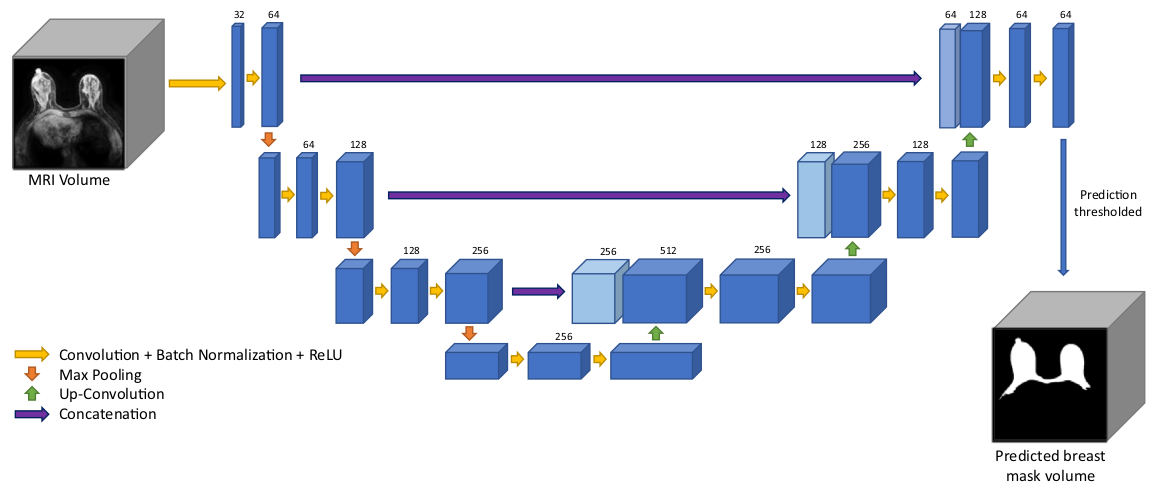
\includegraphics[width=\textwidth]{images/2025-07-07-12-01-04.png} 
	 \caption{Overview dei dati di input e la U-NET usata per la segmentazione del seno.}
    \label{fig:schema_segmentazione_seno_paper}
 \end{figure} 

Il lavoro si distingue per l’approccio rigoroso e riproducibile all’annotazione dei dati: 100 studi MRI, selezionati dal dataset pubblico \textit{Duke Breast Cancer MRI}, sono stati annotati manualmente seguendo criteri ben definiti e validati da radiologi specializzati. Le annotazioni sono tridimensionali e comprendono il tessuto mammario, il FGT e i vasi, un elemento spesso trascurato in studi precedenti.

Dal punto di vista architetturale, il sistema utilizza due reti U-Net in cascata:
\begin{itemize}
\item \textbf{Breast U-Net}, che segmenta il tessuto mammario nell’intero volume MRI.
\item \textbf{FGT-Vessel U-Net}, che utilizza sia il volume MRI che la segmentazione del seno come input per individuare il FGT e i vasi sanguigni.
\end{itemize}

Le performance sono state valutate tramite il coefficiente di similarità di Dice (DSC), ottenendo i seguenti risultati medi sul test set:
\begin{itemize}
\item \hlight{Breast segmentation: DSC = 0.92 (3D), 0.95 (2D)}
\item \hlight{FGT segmentation: DSC = 0.86 (3D), 0.84 (2D)}
\item \hlight{Blood vessels: DSC = 0.65 (3D), 0.53 (2D)}
\end{itemize}

Un elemento innovativo del lavoro è la segmentazione esplicita dei vasi, che ha mostrato impatto significativo nella stima della densità mammaria. In effetti, il volume dei vasi rappresentava in media il 5.7\% del totale dei voxel etichettati come FGT o vasi. Trascurare questo aspetto, come avveniva in studi precedenti, può portare a una sovrastima della densità mammaria.

% \Section{Le Sfide Aperte}
% Nonostante i progressi compiuti, la segmentazione del seno in MRI 3D presenta ancora diverse criticità. Una delle principali è la scarsità di dataset pubblici di grandi dimensioni, soprattutto se confrontata con la disponibilità di dati per altri organi come il cervello o il fegato. Inoltre, i modelli esistenti faticano spesso a generalizzare su dati provenienti da diversi centri medici, a causa delle variazioni tra scanner e protocolli di acquisizione.

% Un altro aspetto critico è l’integrazione di questi strumenti nei workflow clinici quotidiani. Molti modelli, pur offrendo prestazioni elevate in contesti sperimentali, non sono ancora ottimizzati per l’uso in tempo reale o per interagire con i sistemi informativi ospedalieri. Infine, la mancanza di interpretabilità delle predizioni rimane un ostacolo significativo per l’adozione clinica, poiché i medici necessitano di comprendere le basi delle decisioni algoritmiche.

% Questo contesto evidenzia l’importanza di sviluppare soluzioni innovative che affrontino non solo gli aspetti tecnici della segmentazione, ma anche le esigenze pratiche degli operatori sanitari. La pipeline proposta in questo lavoro si inserisce proprio in questo spazio, cercando di colmare alcune delle lacune esistenti attraverso un approccio bilanciato tra accuratezza, efficienza e adattabilità.
\Chapter{Dataset: Duke Breast Cancer MRI}

\Section{Composizione del Dataset}

Il dataset utilizzato durante il tirocinio proviene dal database \hlight{Duke Breast Cancer MRI}, un archivio pubblico contenente immagini DICOM di risonanze magnetiche della mammella. Ogni caso clinico è organizzato in una struttura gerarchica che riflette l'identificativo univoco del paziente e delle relative acquisizioni.

Il dataset è composto da sequenze \hlight{DICOM} tridimensionali, ciascuna rappresentante un'acquisizione volumetrica del seno. In tutti i casi sono disponibili anche annotazioni o maschere segmentate manualmente da esperti, utilizzate come ground truth per il training dei modelli di segmentazione.

Durante la fase di preparazione, le immagini sono state convertite in formato compatibile con MONAI tramite una pipeline di preprocessing, che ha incluso:
\begin{itemize}
    \item il \textbf{caricamento} delle immagini in memoria;
    \item la standardizzazione dell'intensità e il ridimensionamento spaziale;
    \item l'organizzazione dei dati in \textbf{dizionari} contenenti sia l'immagine sia i relativi metadati;
    \item la \textbf{salvataggio} del dataset preprocessato 
\end{itemize}

Per ogni volume è stata mantenuta l'associazione tra immagine e metadati (es. spacing, orientamento, posizione del paziente), necessari per garantire una corretta elaborazione e interpretazione dei dati durante le fasi di training, validazione e inferenza.

L'intero dataset è stato infine suddiviso in tre sottoinsiemi: \hlight{training}, \hlight{validation} e \hlight{test}, rispettando la proporzione e la varietà dei casi clinici per assicurare una valutazione affidabile delle performance del modello.
\Chapter{Configurazione Sperimentale}

Per effettuare gli esperimenti ho avuto la possibilità di utilizzare un \textbf{framework sperimentale} sviluppato dall'ingegner \hlight{Marco Cantone} ~\cite{MarcoCantone}, \textbf{correlatore di questa tesi}. Il cuore del framework risiedeva nella sua capacità di \textbf{astrarre la complessità tipica degli esperimenti di deep learning} attraverso una struttura di configurazione \textbf{gerarchica} e \textbf{intuitiva}. Ogni aspetto cruciale del processo, dal \textbf{preprocessing} dei dati alla \textbf{definizione dell'architettura}, dagli \textbf{iperparametri di training} alle \textbf{metriche di valutazione}, trovava una precisa collocazione nel file \textbf{YAML}.

Uno dei maggiori vantaggi di questo approccio emergeva nella \textbf{fase di validazione incrociata delle ipotesi}. La possibilità di confrontare direttamente diverse varianti architetturali, mantenendo invariati tutti gli altri parametri, ha permesso di isolare con precisione l'impatto di ciascuna scelta progettuale.


Sebbene il framework fornisse una struttura organizzata per gli esperimenti, \textbf{non era dotato di sistemi intelligenti in grado di verificare automaticamente la coerenza logica delle configurazioni}. Spettava quindi a me, durante la definizione dei parametri nel file YAML, assicurarmi che le scelte fossero \textbf{compatibili} tra loro e adatte al contesto. Ad esempio, se impostavo un'architettura progettata per input volumetrici, dovevo verificare manualmente che anche le trasformazioni di preprocessing (come il random padding o il resizing) fossero configurate per operare su tre dimensioni, evitando incongruenze che avrebbero compromesso l'addestramento. 


Allo stesso modo, quando sperimentavo ottimizzatori diversi, dovevo prestare attenzione alla scelta del \textbf{learning rate} e dello \textbf{scheduler}, poiché valori troppo aggressivi potevano \textbf{destabilizzare il training}, mentre quelli troppo conservativi \textbf{rallentavano inutilmente la convergenza}. 

Questo processo richiedeva una costante \textbf{analisi degli errori}: se un esperimento falliva o produceva risultati insoliti, dovevo riesaminare la configurazione YAML per identificare possibili discrepanze, come \textbf{dimensioni di crop incompatibili} con la \textbf{risoluzione del volume} o \textbf{parametri di augmentazione eccessivamente distorti}. La mancanza di validazione automatica ha reso il lavoro più impegnativo, ma mi ha spinto a \textbf{sviluppare una profonda comprensione delle dipendenze tra i vari componenti del sistema}.


\Section{Il file di configurazione YAML}
Il file di configurazione YAML è organizzato in \textbf{sezioni logiche} che definivano ogni aspetto del processo di \textbf{addestramento} e \textbf{valutazione}. Di seguito, analizziamo le componenti principali del file, suddividendolo in sottoinsiemi funzionali.

\Subsection{Struttura generale}
Il file YAML è organizzato in 6 sezioni principali:

\begin{code}{yaml}
# Esempio di struttura generale
TRAINING:
  # parametri di addestramento
TRAIN_TRANSFORM:
  # trasformazioni per il training
TEST_TRANSFORM:
  # trasformazioni per il test
MODEL:
  # architettura del modello
LOSS:
  # funzione di loss
OPTIMIZER:
  # ottimizzatore
\end{code}

\Subsection{Configurazione del training}
La sezione \texttt{TRAINING} definiva i parametri fondamentali:

\begin{code}{yaml}
TRAINING:
  workspace: /path/to/experiment_results
  dataset_root: /path/to/dataset
  valid_size: 0.1  # 10% validation set
  test_size: 0.1   # 10% test set
  train_batch_size: 4
  test_batch_size: 1 
  num_workers: 8    # thread per data loading
  device: cuda:0    # GPU da utilizzare
  epochs: 50        # numero di epoche
  roi_size: [256, 256, 32]  # dimensione regioni di interesse
\end{code}

\Subsection{Trasformazioni dei dati}

Le sezioni \texttt{TRAIN\_TRANSFORM} e \texttt{TEST\_TRANSFORM} specificavano il preprocessing:

\begin{code}{yaml}
TRAIN_TRANSFORM:
  - class: monai.transforms.LoadImaged
    params:
      keys: ['post_2', 'breast']
  - class: monai.transforms.RandSpatialCropSamplesd
    params:
      keys: ['img', 'seg']
      num_samples: 4
      roi_size: [512, 512, 8]
\end{code}


\Subsection{Definizione del modello}
La sezione \texttt{MODEL} configurava l'architettura della rete:

\begin{code}{yaml}
MODEL:
  class: monai.networks.nets.Unet
  params:
    channels: [16, 32, 64]  # canali per ogni livello
    in_channels: 1          # canali input
    out_channels: 2         # canali output
    norm: INSTANCE          # normalizzazione
    spatial_dims: 3         # dimensione spaziale
    strides: [2, 2, 2]      # stride dei livelli
\end{code}


\Subsection{Ottimizzazione e loss}
Le sezioni \texttt{LOSS} e \texttt{OPTIMIZER} controllavano l'addestramento, includendo la funzione di loss e l'ottimizzatore:


\begin{code}{yaml}
LOSS:
  class: monai.losses.DiceFocalLoss
  params:
    weight_dice: 0.7
    weight_ce: 0.3

OPTIMIZER:
  class: torch.optim.AdamW
  params:
    lr: 1e-3               # learning rate
    weight_decay: 1e-3      # regolarizzazione
\end{code}


\Subsection{Post-processing e valutazione}
Le sezioni finali gestivano la valutazione:

\begin{code}{yaml}
METRIC:
  class: monai.metrics.DiceMetric
  params:
    include_background: false
    reduction: mean

POST_PRED:                                                                              
  - class: monai.transforms.AsDiscrete
    params:
      argmax: true
      to_onehot: 2

POST_LABEL:                                                                                 
  - class: monai.transforms.AsDiscrete
    params:
      to_onehot: 2
\end{code}



\Section{Gestione del Logging}

Per ogni esperimento è stato adottato un sistema di \textbf{logging automatico} organizzato in modo da raccogliere tutti gli output generati in una \textbf{cartella dedicata}, con l’obiettivo di garantire tracciabilità, riproducibilità e analisi approfondita dei risultati.

%Struttura delle cartelle
La struttura delle cartelle seguiva uno schema gerarchico, con una cartella principale per ogni esperimento, identificata da un nome univoco basato sulla data e sull'ora di inizio. All'interno di questa cartella, venivano create sottocartelle
per ogni fase del processo di addestramento e valutazione, consentendo una facile navigazione e gestione dei risultati. Ad esempio, la struttura poteva apparire come segue:\\
\begin{minipage}{\textwidth}
\begin{code}{bash}
+-- exp_i/
|   +-- log.txt
|   +-- loss_curve.png
|   +-- metric_curve.png
|   +-- best_model.pth
|   +-- predictions/
|       +-- case_001/
|       |   +-- slice_01.png
|       |   +-- slice_02.png
|       |   +-- ...
|       +-- case_002/
|       |   +-- slice_01.png
|       |   +-- ...
|       +-- ...
\end{code}
\end{minipage}
\\


Ogni cartella conteneva le seguenti informazioni:

\begin{itemize}
\item Un file \texttt{log.txt} contenente tutte le stampe console (\texttt{print}) prodotte durante il training. In questo file venivano riportati:
\begin{itemize}
\item la \textbf{loss di training} e \textbf{validazione} per epoca;
\item le \textbf{metriche di valutazione} (es. \textbf{Dice score});
\item eventuali \textbf{messaggi diagnostici}.
\end{itemize}
\item Due \textbf{grafici} in formato immagine (\texttt{.png}):
\begin{itemize}
    \item il grafico della \textbf{curva della loss} per epoca;
    \item il grafico della \textbf{metrica} per epoca.
\end{itemize}

\item Il file del \textbf{modello salvato} (\texttt{.pth}), che rappresenta lo \textbf{stato della rete al miglior checkpoint}.

\item Una sottocartella \texttt{predictions/} contenente, per ogni caso del \textbf{test set}, le \textbf{immagini salvate slice per slice}. Ogni immagine mostrava sovrapposte:
\begin{itemize}
    \item \textbf{l’immagine originale della MRI dell'i-esima slice}
    \item la \textbf{ground truth} dell'i-esima slice
    \item la \textbf{predizione generata dal modello} dell'i-esima slice
\end{itemize}

\end{itemize}

Questa struttura ha permesso non solo di \textbf{monitorare l’andamento dell’addestramento}, ma anche di effettuare \textbf{confronti qualitativi tra modelli diversi} e analizzare visivamente i punti di \textbf{forza} e \textbf{debolezza} della rete. Inoltre, la separazione per cartelle ha reso semplice la gestione di esperimenti multipli e il confronto sistematico tra diverse configurazioni di training.
\Chapter{Esperimenti}


\Section{Introduzione}
Sono stati condotti diversi esperimenti, cercando di variare gli aspetti della configurazione del modello e del processo di addestramento, al fine di ottimizzare le prestazioni nella segmentazione delle immagini mammografiche. Si è cercato di \textbf{cambiare gli iperparametri uno alla volta}, mantenendo costanti gli altri, per isolare l'impatto di ciascuna modifica. 

Lo sviluppo di un sistema di segmentazione automatica efficace richiede non solo un’adeguata progettazione architetturale, ma anche un attento processo di \textbf{ottimizzazione sperimentale}, che tenga conto delle molteplici variabili che influenzano l’apprendimento del modello. In questo capitolo viene descritto in dettaglio il percorso iterativo seguito, che ha portato a una \textbf{progressiva evoluzione del modello} fino a raggiungere \textbf{performance soddisfacenti}.

\Subsection{Nota sulle Valutazioni}
Nei primi \textbf{16 esperimenti}, la valutazione sul \textbf{test set} è stata effettuata utilizzando le \textbf{immagini trasformate}, ovvero mantenendo le dimensioni e le modifiche introdotte durante il preprocessing (incluso il resize). A partire dall'esperimento \textbf{17}, invece, è stata applicata una \textbf{trasformazione inversa} (in particolare il resize inverso) alle ground truth, riportandole alle dimensioni originali. Questo ha permesso una valutazione più corretta e realistica delle performance, evitando possibili distorsioni dovute alle trasformazioni di preprocessing.

\begin{table}[!ht]
    \begin{center}
    \begin{NiceTabular}{rrr}[rules/color={gray!90},rules/width=1pt]
        \CodeBefore
        \rowcolors{1}{black!5}{}
        \rowcolors{3}{blue!5}{}
        \Body
        \toprule
        \textbf{EXP} & \textbf{Architettura} & \textbf{Parametri Chiave} \\
        \midrule
        1-3 & U-Net 3D & Canali [16,32,64,128] \\
        4-10 & U-Net 3D & Canali [16,32,64,128,256] \\
        12,13 & SliceU-Net 2D & Approccio 2D slice-based \\
        14-21 & U-Net 3D & Varianti profondità/canali \\
        20 & Attention U-Net 3D & Meccanismo di attention \\
        \bottomrule
    \end{NiceTabular}
\end{center}
    \caption{Configurazioni principali dei modelli sperimentali con architetture e parametri chiave.}
    \label{tab:config_modelli}
\end{table}




\Section{Impostazione degli Esperimenti}

Gli esperimenti sono stati condotti in \textbf{maniera incrementale}, seguendo una filosofia di \hlight{ottimizzazione guidata da evidenze}, nella quale ciascuna modifica introdotta agli iperparametri o alla pipeline di preprocessing è stata motivata da osservazioni emerse negli esperimenti precedenti. Tutte le prove sono state \textbf{documentate} e \textbf{monitorate} con precisione.

Per garantire la coerenza e individuare possibili problemi, è stato anche necessario implementare un sistema di \hlight{debugging interno} tramite Python, includendo \textbf{stampe delle dimensioni dei tensori nei momenti chiave} del forward pass e salvataggi intermedi delle immagini durante il training. Questo approccio ha \hlight{permesso di identificare rapidamente errori legati a mismatch dimensionali, problemi nella gestione della normalizzazione, o trasformazioni incoerenti nei dati di input/output.}

\Section{Evoluzione Architetturale e Tuning degli Iperparametri}

Il \textbf{primo esperimento} (tab. \ref{tab:exp1_config}) ha costituito la \textbf{base di partenza}, con una configurazione \textbf{standard della rete U-Net tridimensionale}, con \textbf{4 blocchi convoluzionali} (\texttt{channels: [16, 32, 64, 128]}), \textbf{normalizzazione batch}, e un \textbf{resize uniforme} applicato a tutte le immagini. Con questa configurazione, è stato ottenuto un \hlight{Dice score sul test set pari a 0.7894}.

\begin{table}[H]
    \begin{center}
        \begin{NiceTabular}{rc}[rules/color={gray!90},rules/width=1pt]
            \CodeBefore
            \rowcolors{1}{black!5}{}
            \rowcolors{3}{blue!5}{}
            \Body
            \toprule
            \textbf{Parametro}      & \textbf{Valore}                                \\
            \midrule
            \textbf{Architettura} & U-Net 3D standard con 4 blocchi convoluzionali \\
            \textbf{Canali} & [16, 32, 64, 128] \\
            \textbf{Normalizzazione} & Batch normalization \\
            \textbf{Resize} & Uniforme su tutte le immagini \\
            \textbf{Dice score (test set)} & 0.7894 \\
            \bottomrule
        \end{NiceTabular}
    \end{center}
	\caption{Configurazione del primo esperimento (baseline) con architettura U-Net 3D e risultati ottenuti.}
	\label{tab:exp1_config}
\end{table}


Il \textbf{passo successivo} ha previsto un \textbf{aumento del learning rate} dell’ottimizzatore \textbf{Adam}, passando da \textbf{0.0005} a \textbf{0.005}. Questo semplice cambiamento ha prodotto un \hlight{incremento della metrica di circa +1.17\%,} suggerendo che la rete era in grado di \hlight{convergere più rapidamente in presenza di un gradiente iniziale più marcato}. Da qui è emersa l’intuizione che la rete potesse beneficiare anche di una \hlight{maggiore profondità}: il \textbf{terzo} e il \textbf{quarto} esperimento (tab. \ref{tab:exp3-4_results}) \hlight{hanno confermato questa ipotesi, mostrando miglioramenti crescenti in validazione e test} con l’introduzione di un ulteriore blocco (\texttt{channels: [16, 32, 64, 128, 256]}), fino a raggiungere \hlight{0.8597 sul test set} e \hlight{0.8569 sul validation set}.

\begin{table}[H]
    \centering
	\begin{NiceTabular}{rc}[rules/color={gray!90},rules/width=1pt]
		\CodeBefore
		\rowcolors{1}{black!5}{}
		\rowcolors{3}{blue!5}{}
		\Body
		\toprule
		\textbf{Parametro} & \textbf{Valore} \\
		\midrule
		\textbf{Architettura} & U-Net 3D profonda con 5 blocchi convoluzionali \\
		\textbf{Canali} & [16, 32, 64, 128, 256] \\
		\textbf{Normalizzazione} & Batch normalization \\
		\textbf{Dice score (test)} & 0.8597 \\
		\textbf{Dice score (validazione)} & 0.8569 \\
		\bottomrule
	\end{NiceTabular}
	\caption{Risultati degli esperimenti 3-4 con architettura U-Net 3D più profonda. L'aggiunta di un quinto blocco convoluzionale ha portato a significativi miglioramenti nelle metriche.}
	\label{tab:exp3-4_results}
\end{table}

A partire dal \textbf{quinto esperimento} (tab. \ref{tab:exp5_comparative}) è stata esplorata una \textbf{combinazione di modifiche strutturali}, tra cui il passaggio da \textbf{Adam} ad \hlight{AdamW}, il cambiamento della \textbf{normalizzazione} da \textbf{Batch} a \hlight{Instance} e l’utilizzo di una \textbf{loss} \textbf{composita} (\hlight{Focal} + \hlight{Dice} \hlight{Loss}), ciascuna ponderata per gestire in modo bilanciato gli squilibri tra le classi. Questa configurazione ha prodotto \hlight{ottimi risultati in validazione (0.8623) e (0.8597) sul test set}.
\begin{table}[H]
    \centering
    \begin{NiceTabular}{rl}[rules/color={gray!90},rules/width=1pt]
        \CodeBefore
        \rowcolors{1}{black!5}{}
        \rowcolors{3}{blue!5}{}
        \Body
        \toprule
        \textbf{Componente} & \textbf{Modifica} \\
        \midrule
        \textbf{Ottimizzazione} & Sostituzione Adam → AdamW \\
        \textbf{Normalizzazione} & Batch → Instance \\
        \textbf{Loss function} & Dice → DiceFocal ($\lambda$ =0.7/0.3) \\
        \textbf{Metriche} & $\Delta$ Valid +3.1\%, $\Delta$ Test +0.32\% \\
        \textbf{Risultati} & Valid: 0.8623, Test: 0.8597 \\
        \bottomrule
    \end{NiceTabular}
    \caption{Analisi comparativa delle modifiche introdotte dall'EXP 5. Tutti i cambiamenti hanno contribuito al miglioramento delle performance.}
    \label{tab:exp5_comparative}
\end{table}


Nei \textbf{successivi esperimenti}, si è indagata ulteriormente la sensibilità del modello al \textbf{learning rate}, che era stato inizialmente portato troppo in basso (\texttt{0.0001}). Ripristinando un valore intermedio (\texttt{0.001}), il \hlight{Dice score sul test è aumentato di oltre il 3\%.} Parallelamente, l’introduzione di una strategia di \hlight{learning rate scheduling  (LinearWarmupCosineAnnealingLR)} (fig. \ref{fig:learning_rate_scheduling}) ha portato a \hlight{miglioramenti più modesti ma stabili}.

\begin{figure}[H] 
  	\centering 
 	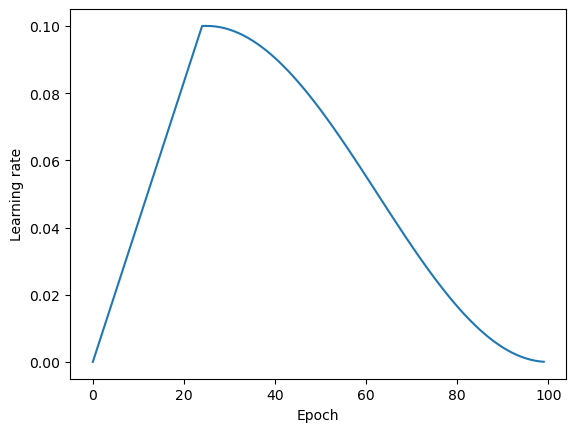
\includegraphics[width=.6\textwidth]{images/2025-07-12-11-28-31.png} 
    \caption{Andamento del learning rate durante il training, con warmup iniziale e successiva discesa coseno.}
    \label{fig:learning_rate_scheduling}
 \end{figure} 



 


Una seconda linea di sperimentazione ha riguardato il \textbf{trattamento dimensionale} delle immagini. Portando la dimensione da \textbf{(384x384)} a \hlight{(512x512)}, si è osservato un ulteriore \hlight{miglioramento della metrica}. Al contrario, strategie basate esclusivamente sul \textbf{padding}, o su un \textbf{mix di resize e padding}, hanno avuto un effetto \hlight{negativo} sulle performance, portando a un crollo significativo della metrica nel \textbf{nono} e \textbf{decimo} esperimento fino a \hlight{0.7576 sul test set} e \hlight{0.0816 in validazione}. 

\begin{table}[H]
    \centering
    \begin{NiceTabular}{rccc}[rules/color={gray!90},rules/width=1pt]
        \CodeBefore
        \rowcolors{1}{black!5}{}
        \rowcolors{3}{blue!5}{}
        \Body
        \toprule
        \textbf{Configurazione} & \textbf{Dimensione} & \textbf{Test Dice} & \textbf{Valid Dice} \\
        \midrule
        \textbf{Baseline} & 384×384 & 0.7894 & 0.7920 \\
        \rowcolor{green!5}
        \textbf{Full Resize} & 512×512 & \textbf{0,8878} & \textbf{0,8934} \\
        \rowcolor{red!5}
        \textbf{Solo Padding} & 512×512 & 0.7576 & 0.8160 \\
        \textbf{Mix Strategie} & Variabile & 0,8857 &  0,8848 \\
        \bottomrule
    \end{NiceTabular}
    \caption{Confronto sistematico degli approcci dimensionali. I valori mostrano come il resize completo produca i migliori risultati, mentre il padding peggiora le performance.}
    \label{tab:dimension_comparison}
\end{table}


\Section{Strategia Alternativa: Approccio 2D e Architettura SliceUNet}

In seguito a questi risultati, è stata sperimentata una \hlight{nuova strategia}, volta a esplorare un \hlight{approccio 2D} invece che 3D. Questo ha richiesto l’adozione di una \textbf{ROI size} di tipo \textbf{(512, 512, 1)}, accompagnata da una trasformazione \texttt{RandSpatialCropSamplesd} e da un’opportuna gestione del padding. Per rendere l’intera pipeline compatibile con questo formato, è stata definita un’architettura \hlight{SliceUNet personalizzata}, progettata per operare su \textbf{singole slice bidimensionali} mantenendo il supporto volumetrico per \textbf{l’aggregazione del risultato finale}.

\begin{code}{python}
class SliceUNet(nn.Module):
    def __init__(self, in_channels, out_channels, 
                channels, norm, strides, spatial_dims=2):
        super(SliceUNet, self).__init__()
        self.Unet2D = monai.networks.nets.UNet(
            spatial_dims=spatial_dims,
            in_channels=in_channels,
            out_channels=out_channels,
            channels=channels,
            strides=strides,
            norm= norm,
        )
    def forward(self, x):
        x = self.Unet2D(x[...,0]) 

        return x[..., None]
\end{code}



I primi esperimenti con \textbf{SliceUNet} hanno ottenuto \hlight{risultati interessanti}: partendo da \textbf{0.628}, si è passati a \hlight{0.7808, in test}, modificando la strategia di preprocessing da \textbf{padding} a \hlight{resize}. Tuttavia, nonostante \textbf{l’eleganza} e la \textbf{semplicità computazionale} di questo approccio, i risultati \hlight{non hanno raggiunto i livelli di accuratezza ottenibili con la versione 3D}.

\Section{Ritorno all’approccio 3D: Affinamento e Validazione}

Per questo motivo, \textbf{l’attenzione è tornata su modelli tridimensionali}, testando configurazioni diverse di \texttt{roi\_size} (ad esempio, \texttt{(512x512x16)}) e nuove combinazioni architetturali. \hlight{Esperimenti successivi hanno mostrato che aumentando la profondità lungo l’asse z} e spingendo il numero di \hlight{epoche a 150}, si potevano ottenere performance vicine a \hlight{0.8863 in test}, che \hlight{costituivano il massimo assoluto fino a quel punto.}

\begin{table}[H]
    \centering
    \begin{NiceTabular}{rccc}[rules/color={gray!90},rules/width=1pt]
        \CodeBefore
        \rowcolors{1}{black!5}{}
        \Body
        \toprule
        \textbf{Tipo} & \textbf{Parametri Chiave} & \textbf{Test Dice} & \textbf{$\Delta$} \\
        \midrule
        \rowcolor{red!3}
        \textbf{2D Base} 
        & SliceUNet, padding, 50 epoche & 0.628 & \color{gray}{-} \\
        \rowcolor{yellow!3}
        \textbf{2D Migliorato} 
        & SliceUNet, resize $512\times512$  & 0.7808 & \color{green!70!black}{\textbf{↑24.3\%}} \\
        \rowcolor{green!8}
        \textbf{3D Intermedio} 
        & U-Net, ROI $512\times512\times16$ & 0.8668 & \color{green!70!black}{\textbf{↑38.0\%}} \\
        \rowcolor{blue!8}
        \textbf{3D Ottimale} 
        & +150 epoche, asse z profondo & \cellcolor{blue!10}\textbf{0.8863} & \cellcolor{blue!10}\color{blue!80!black}{\textbf{↑41.1\%}} \\
        \bottomrule
    \end{NiceTabular}
    \caption{Progressione prestazionale con scala cromatica: dal rosso (baseline) al blu (miglior risultato). I $\Delta$ verdi mostrano il miglioramento cumulativo, mentre il blu evidenzia il picco prestazionale (+41.1\% rispetto alla baseline).}
    \label{tab:3d_color_progression}
\end{table}



%   ┌───────────────────────┐
%   │ SONO ARRIVATO FIN QUI │
%   └───────────────────────┘


\Section{Nuovo approccio di Valutazione}
Un \hlight{aspetto critico} che è emerso in questa fase è stato \textbf{il modo in cui le predizioni venivano valutate}. In effetti, l’adozione di tecniche di preprocessing alterava la struttura delle label, rendendo la metrica poco rappresentativa. È stata quindi introdotta una \textbf{pipeline di trasformazioni inverse} nella fase di test, per riportare le predizioni allo spazio originale e confrontarle correttamente con le etichette intonse.

\begin{code}{python}
if isinstance(test_loader.dataset.transform, Compose) 
            and any(isinstance(tr, Resized) 
            for tr in test_loader.dataset.transform.transforms):
    val_outputs = [Resized(keys="img", spatial_size=original_shape, 
                mode="nearest")
                    ({"img": i})["img"] for i in val_outputs]
\end{code}

% Con questa nuova metodologia di test, sono stati ripetuti alcuni esperimenti precedenti. Sebbene i risultati apparissero \textbf{lievemente più bassi in termini assoluti}, la loro \textbf{affidabilità era notevolmente superiore}. In questo contesto, nuove architetture come l’\textbf{Attention U-Net} e reti con struttura compressa ma profonda hanno ottenuto risultati significativi, culminando nel ventunesimo esperimento con un Dice score pari a \textbf{0.9124}, il valore più alto registrato sull’intero test set.

Con questa nuova metodologia di test, sono stati ripetuti alcuni esperimenti precedenti, mantenendo \textbf{invariati l’architettura}, la \textbf{configurazione degli iperparametri} e il \textbf{preprocessing}, ma modificando il modo in cui veniva eseguita la valutazione sul test set. L’introduzione delle \textbf{trasformazioni inverse}, ha evidenziato una \textbf{differenza sostanziale} tra le metriche riportate in precedenza e quelle ricalcolate in condizioni più rigorose. Ad esempio, l’esperimento \textbf{16}, che con il metodo di valutazione originale aveva raggiunto un \textbf{Dice score di 0.8863}, è stato ripetuto come esperimento \textbf{20}, ottenendo un valore \hlight{ridotto di 0.8567.} 

Nonostante questa lieve flessione nei valori assoluti, la nuova metodologia \hlight{ha reso i confronti tra modelli molto più affidabili}. Alcune architetture, che in precedenza sembravano promettenti ma erano in realtà favorite da un confronto distorto, hanno rivelato prestazioni inferiori alle attese. %Al contrario, modelli più solidi e coerenti, come l’\textbf{Attention U-Net} testato nell’esperimento \textbf{19}, hanno confermato la loro efficacia anche sotto il nuovo regime di valutazione, raggiungendo un Dice score di \textbf{0.8415} dopo 150 epoche di addestramento.

\Subsection{L’Attention U-Net}

L’\textbf{Attention U-Net} (fig. \ref{fig:attention_unet}) rappresenta una naturale estensione della classica architettura \textbf{U-Net}, progettata per migliorare la capacità del modello di \textbf{concentrarsi sulle regioni di interesse  più rilevanti all’interno dell’immagine}. Introdotta da \textbf{Oktay et al. nel 2018} \cite{oktay2018attention}, questa variante si basa sull’integrazione di \textbf{meccanismi di attenzione spaziale} nei percorsi di \textbf{skip connection} tra \textbf{encoder} e \textbf{decoder}. L’obiettivo principale è quello di guidare la rete \textbf{nell’enfatizzare le strutture salienti} e nel \textbf{sopprimere attivamente le attivazioni inutili} o irrilevanti, soprattutto in contesti caratterizzati da alta complessità anatomica o forte squilibrio tra classi.

Nella \textbf{U-Net tradizionale}, le informazioni a bassa risoluzione estratte dall’encoder vengono concatenate direttamente con i feature map corrispondenti del decoder. Tuttavia, questo approccio assume che tutte le regioni abbiano pari rilevanza informativa, ignorando il fatto che non tutte le porzioni dell’immagine contribuiscono in egual misura alla segmentazione finale. \textbf{L’Attention U-Net} introduce quindi un \textbf{modulo di attenzione} che agisce come un \textbf{filtro “intelligente”:} prima della concatenazione, il modello valuta l’importanza di ciascuna regione mediante un \textbf{gating mechanism}, che calcola \textbf{mappe di attenzione} specifiche per ogni livello di \textbf{skip connection}.

\begin{figure}[H] 
  	\centering 
 	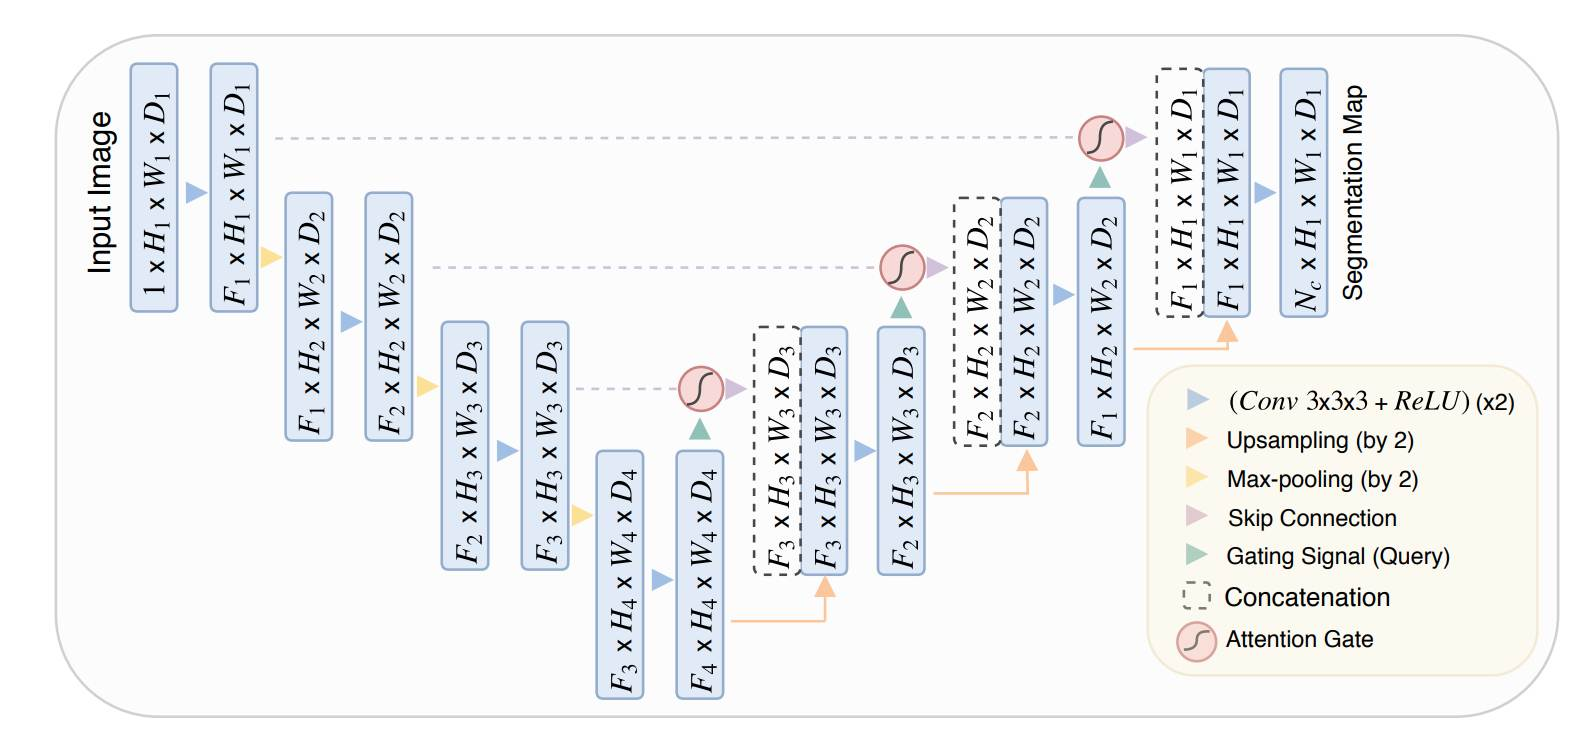
\includegraphics[width=.8\textwidth]{images/2025-07-22-14-33-52.png} 
    \caption{Schema dell’Attention U-Net. Le frecce indicano il flusso di informazioni tra i moduli di encoder e decoder, con l’integrazione del modulo di attenzione.}
    \label{fig:attention_unet}
 \end{figure} 
Dal punto di vista implementativo, il modulo di attenzione riceve in input due segnali: da un lato, \textbf{le feature provenienti dal livello encoder} (contenenti informazione spaziale locale); dall’altro, \textbf{i segnali di gating dal decoder} (contenenti informazione semantica più astratta). L’interazione tra questi due flussi genera una \textbf{mappa di attenzione}, applicata tramite moltiplicazione ai tensori encoder, prima della loro trasmissione al decoder. In questo modo, il decoder riceve solo le informazioni più rilevanti per la predizione finale.

Nel contesto del presente lavoro, \textbf{nonostante un aumento moderato della complessità computazionale}, il modello \hlight{ha mostrato buone performance}, raggiungendo un \hlight{Dice score pari a 0.8415} nell’esperimento dedicato.

\Section{Esperimento Finale}

Il punto culminante di questa fase è stato rappresentato dall’esperimento \textbf{21}, in cui è stata utilizzata una \hlight{U-Net profonda con cinque livelli e stride finale lungo l’asse z pari a 1}. L’input adottava una ROI size tridimensionale pari a $(512, 512, 8)$, e il training è stato prolungato fino a \hlight{200 epoche} (fig. \ref{fig:losses} e fig. \ref{fig:metrics}). 

\begin{minipage}{.48\textwidth}
    \begin{figure}[H] 
        \centering 
        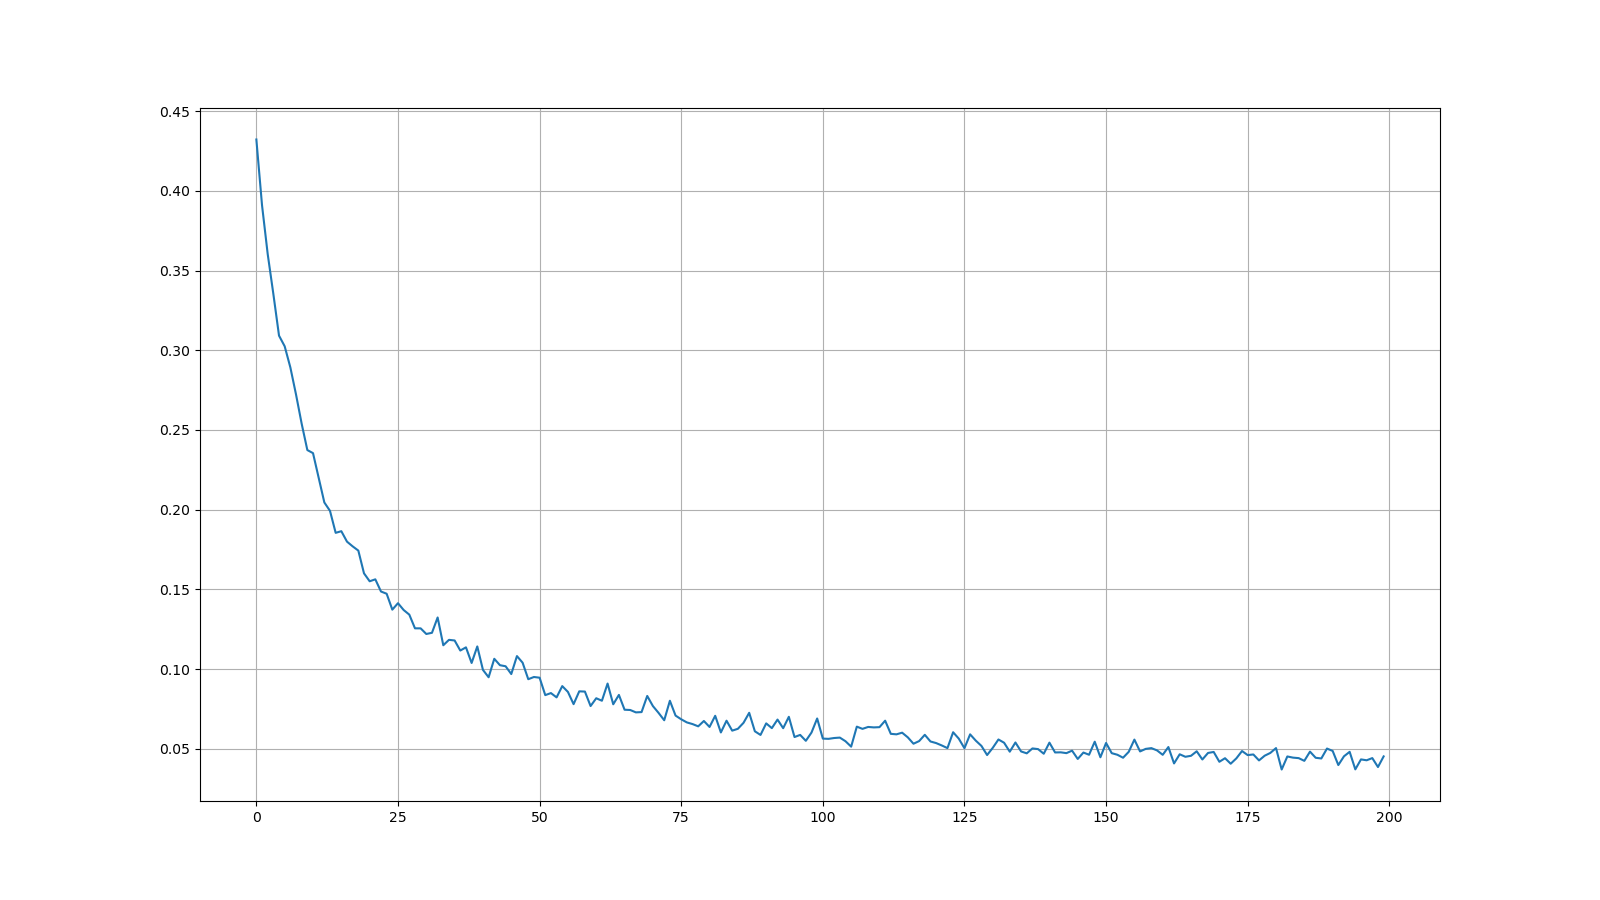
\includegraphics[width=\textwidth]{figures/losses.png} 
        \caption{Andamento delle funzioni di loss durante il training dell’esperimento finale(EXP 21).}
        \label{fig:losses}
    \end{figure} 
\end{minipage}
\hfill
\begin{minipage}{.48\textwidth}
    \begin{figure}[H] 
        \centering 
        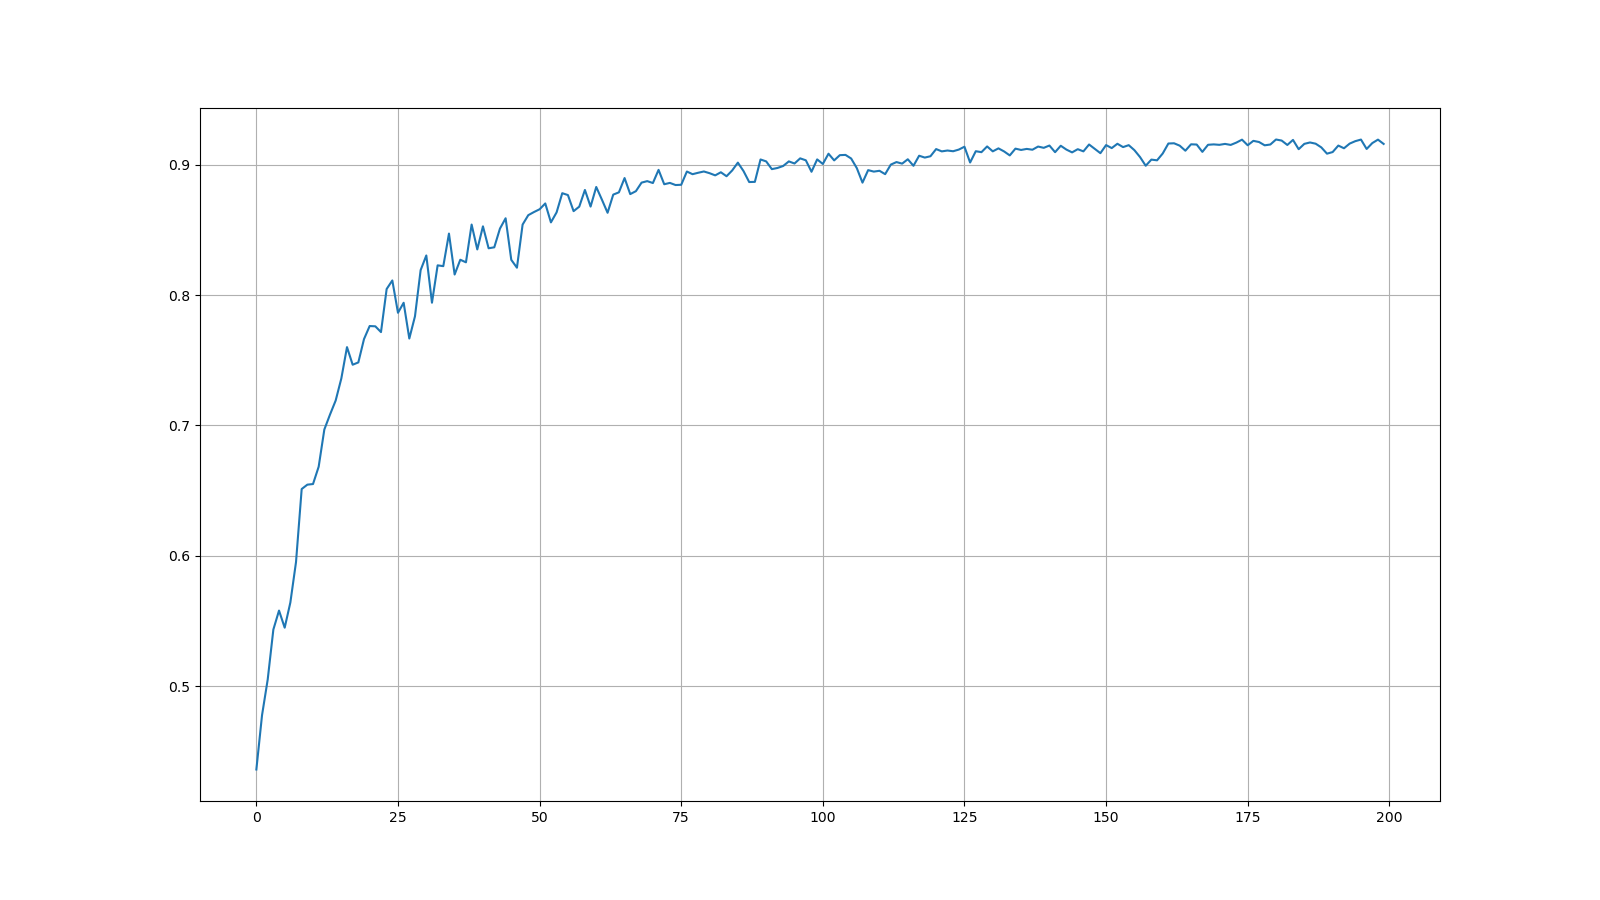
\includegraphics[width=\textwidth]{figures/metrics.png} 
        \caption{Andamento delle metriche di valutazione durante il training dell’esperimento finale(EXP 21).}
        \label{fig:metrics}
    \end{figure} 
\end{minipage}


\begin{figure}[H] 
  	\centering 
 	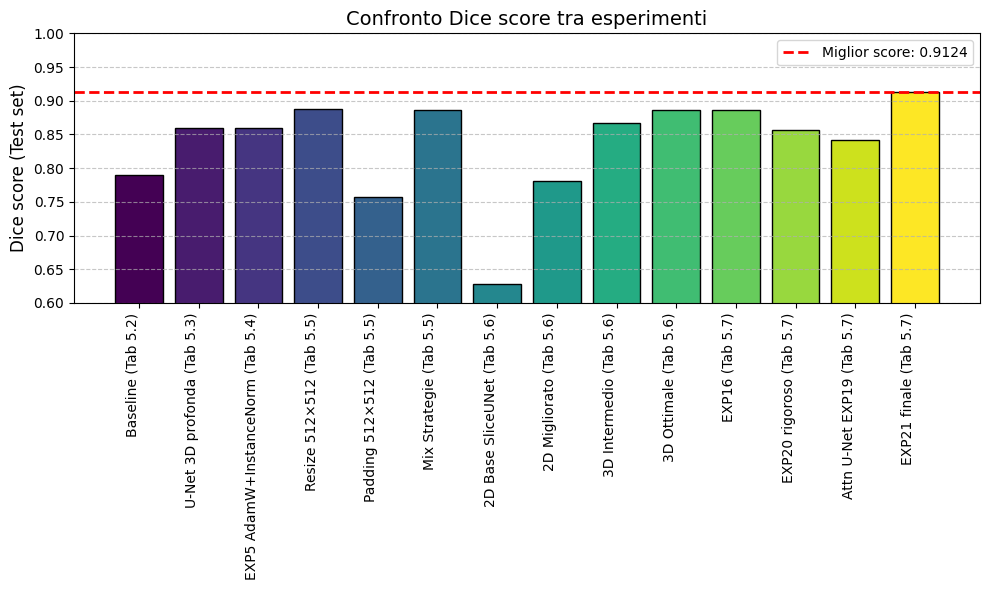
\includegraphics[width=\textwidth]{images/2025-08-19-16-09-18.png} 
    \caption{Confronto Dice score tra tutti gli esperimenti effettuati.}
 \end{figure} 

In queste condizioni, \hlight{il modello ha raggiunto un Dice score pari a 0.9124} (fig. \ref{fig:metrics}), \hlight{il valore più alto registrato su tutto il test set} (fig. \ref{fig:final_segmentation_examples}). Questo risultato rappresenta non solo il successo di una specifica configurazione, ma anche la validazione dell’intero \textbf{processo di ottimizzazione}, culminato in un \textbf{modello accurato}, \textbf{robusto} e valutato con \textbf{criteri metodologicamente solidi}.


\begin{table}[H]
\centering
\begin{NiceTabular}{rlccc}[rules/color={gray!85},rules/width=0.8pt]
\CodeBefore
\rowcolors{1}{}{gray!3}
\Body
\toprule
\textbf{EXP} & \textbf{Configurazione} & \textbf{Dice} & \textbf{$\Delta$} & \textbf{Note} \\
\midrule
16 & Config. originale & 0.8863 & \color{red}{-3.3\%} & Sovrastima precedente \\
20 & Stessa config. + val. rigorosa & 0.8567 & \color{gray}{0\%} & Benchmark corretto \\
19 & Attention U-Net & 0.8415 & \color{red}{-1.8\%} vs 20 & Robustezza verificata \\
\rowcolor{blue!7}
21 & U-Net avanzato & 0.9124 & \color{teal}{+6.5\% vs 20} & Nuovo state-of-the-art \\
\bottomrule
\end{NiceTabular}
\caption{Analisi dettagliata dei risultati finali. La colonna $\Delta$ mostra: per EXP 16 la sovrastima rispetto alla nuova metodologia, per EXP 19-21 la variazione rispetto al benchmark corretto (EXP 20).}
\label{tab:final_results_detailed}
\end{table}



\begin{figure}[H]
    \centering
    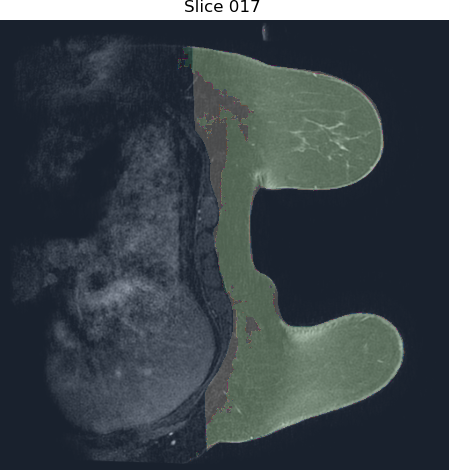
\includegraphics[width=0.40\textwidth]{figures/slice_017.png} 
    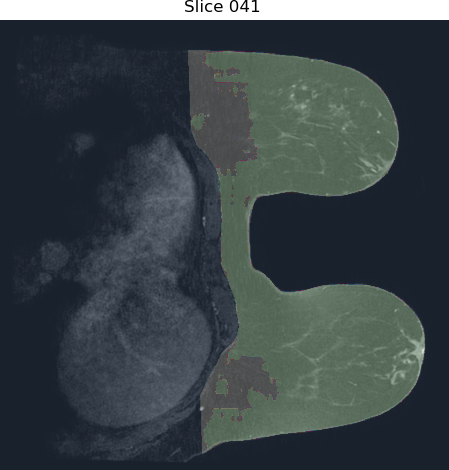
\includegraphics[width=0.40\textwidth]{figures/slice_041.png} 
    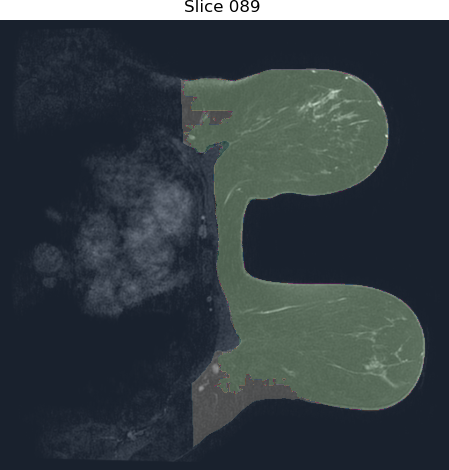
\includegraphics[width=0.40\textwidth]{figures/slice_089.png} 
    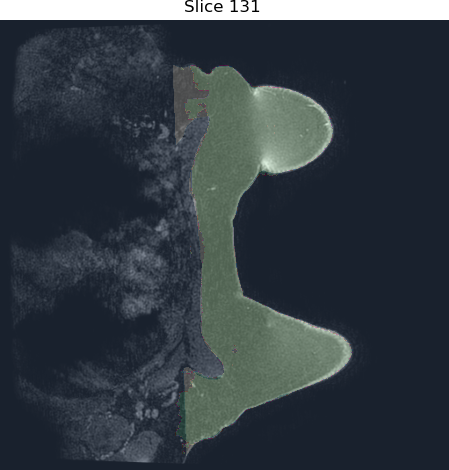
\includegraphics[width=0.40\textwidth]{figures/slice_131.png} 
    \caption{Esempi di segmentazione ottenuti con il modello finale (EXP 21). Le immagini mostrano le predizioni su diverse slice del test set, evidenziando la capacità del modello di identificare correttamente le aree di interesse.}
    \label{fig:final_segmentation_examples}
\end{figure}

\Subsection{Post-processing morfologico: operazione di Closing}

Al termine dell’addestramento del modello finale (EXP~21), è stata introdotta una fase opzionale di \textbf{post-processing morfologico} sulle maschere di segmentazione prodotte, con l’obiettivo di correggere eventuali discontinuità e imperfezioni residue lungo i margini delle strutture segmentate.

L’operazione applicata è il \textbf{closing morfologico} (\emph{dilatazione seguita da erosione}). Questo tipo di trasformazione è comunemente utilizzato per \textbf{colmare piccoli vuoti} all’interno delle regioni segmentate, \textbf{uniformare i bordi} delle maschere e \textbf{migliorare la connettività} delle strutture anatomiche in presenza di interruzioni puntuali.


L'implementazione è stata realizzata creando una funzione custom in Python che applica il closing morfologico su ciascuna maschera di segmentazione generata dal modello. La funzione utilizza la libreria \texttt{scikit-image} per eseguire le operazioni morfologiche, specificando un \textbf{kernel di dimensione fissata dal parametro in ingresso}:

\begin{code}{python}
from scipy.ndimage import binary_closing
from monai.transforms import MapTransform
import torch
import numpy as np

class MorphologicalClosing():
    def __init__(self, dim=12):
        self.dim = dim
        self.structure = np.ones((self.dim, self.dim, self.dim), dtype=bool)
    def __call__(self, x):
        device = x.device if isinstance(x, torch.Tensor) else torch.device('cpu')
        # convert to numpy
        if isinstance(x, torch.Tensor):
            x = x.cpu().numpy()
        # remove first dimension
        x = x.squeeze(0) if x.ndim > 3 else x
        closed_np = binary_closing(x, structure=self.structure)
        # re-add first dimension
        closed_np = closed_np[None, ...]
        # convert back to tensor and move to original device
        closed_tensor = torch.tensor(closed_np, dtype=torch.float32, 
                                    device=device)
        return closed_tensor
\end{code}
Sono state testate diverse dimensioni per il \textbf{kernel size} dell’operazione di closing, variando il parametro tra valori compresi tra 6 e 16. L’analisi sistematica ha mostrato che la dimensione ottimale era pari a \hlight{10}, che garantiva il miglior compromesso tra \textbf{uniformità dei bordi} e \textbf{preservazione dei dettagli anatomici}, evitando sia un’eccessiva erosione sia la formazione di artefatti.

\begin{figure}[H] 
  	\centering 
 	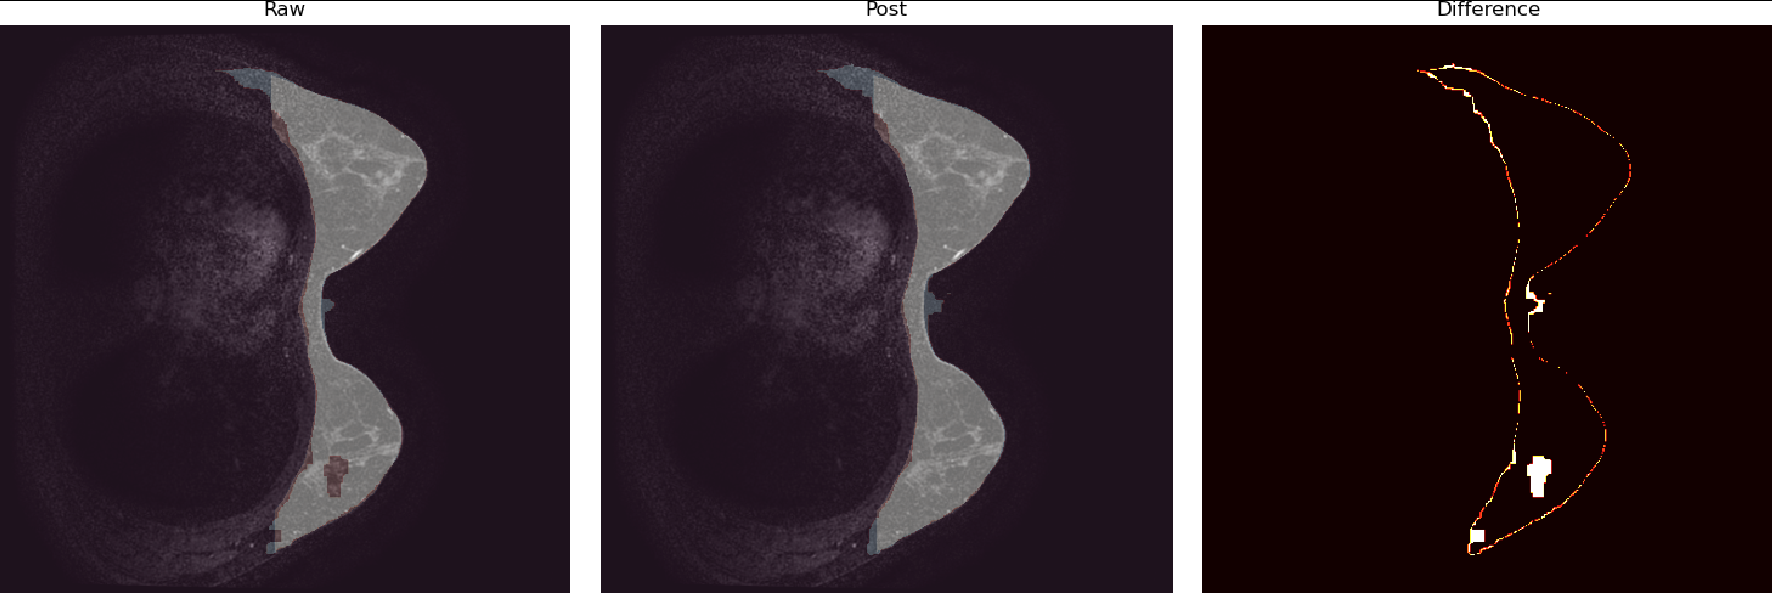
\includegraphics[width=\textwidth]{images/2025-08-08-18-52-24.png} 
    \caption{Esempio di segmentazione prima e dopo l'applicazione del closing morfologico. Le immagini mostrano come il closing migliori la coesione delle strutture segmentate, eliminando piccole discontinuità e rendendo le maschere più uniformi.}
    \label{fig:closing_example}
 \end{figure} 

L’effetto del closing (fig. \ref{fig:closing_example}) è stato valutato rieseguendo la metrica di \textbf{Dice score} sul \emph{test set}. Il modello finale, che in fase di validazione rigorosa aveva raggiunto un valore di \textbf{0.9124}, \hlight{ha beneficiato di un incremento fino a 0.9161} dopo il post-processing. Questo risultato conferma che, pur trattandosi di un miglioramento numericamente modesto \textbf{(\(+0.0037\)),} \hlight{l’operazione di closing ha contribuito a rifinire ulteriormente le maschere, portando a un output visivamente più coerente e clinicamente più fruibile.}




\Chapter{Conclusioni}


\Section{Sintesi del Percorso Sperimentale}

L’analisi sperimentale condotta ha evidenziato che il successo di una pipeline di segmentazione non dipende da un singolo fattore, bensì dall’interazione armonica tra \textbf{scelte architetturali}, \textbf{strategie di preprocessing}, \textbf{criteri di valutazione} e \textbf{robustezza del training}. Ogni esperimento ha rappresentato un passo incrementale verso una maggiore comprensione del comportamento del modello, contribuendo alla costruzione di una soluzione \textbf{affidabile}, \textbf{generalizzabile} e potenzialmente \textbf{integrabile} in contesti clinici reali.

Il percorso si è rivelato altamente \textbf{iterativo} e \textbf{evidence-based}, partendo da una configurazione di base e introducendo, con rigore sperimentale, modifiche mirate al \textbf{learning rate}, alla \textbf{funzione di loss}, al tipo di \textbf{normalizzazione}, alla \textbf{profondità architetturale}, fino a giungere a una configurazione finale profondamente ottimizzata. Particolarmente significativo è stato l’inserimento di una strategia di \textbf{validazione con trasformazioni inverse}, che ha garantito confronti fedeli tra predizioni e maschere originali, migliorando l’affidabilità delle metriche ottenute.

\Section{Risultato Finale e Implicazioni Cliniche}

Il modello finale, sviluppato \textbf{nell’esperimento 21}, ha raggiunto un \hlight{Dice score di 0.9124, arrivando fino a un Dice score di 0.9161 con il closing morfologico finale}. Dimostrando così un'elevata accuratezza predittiva. Il valore di questa performance risiede non solo nella metrica in sé, ma nella sua coerenza con una pipeline sperimentale \textbf{solida}, \textbf{riproducibile} e \textbf{scientificamente fondata}.

Dal punto di vista clinico, i risultati ottenuti hanno implicazioni rilevanti. Automatizzare la \textbf{segmentazione del tessuto mammario}, del \textbf{fibroghiandolare (FGT)} e dei \textbf{vasi sanguigni} consente di ridurre la \textbf{variabilità inter-operatore}, migliorare la \textbf{velocità di refertazione} e supportare nuove forme di \textbf{analisi quantitativa}. In particolare, la stima automatizzata della \textbf{densità mammaria} può influenzare in modo diretto la \textbf{valutazione del rischio oncologico}, abilitando percorsi diagnostici più personalizzati e precoci.

Inoltre, la presenza di maschere segmentate consente di contestualizzare meglio le eventuali lesioni, potenziando strumenti di \textbf{localizzazione assistita} e agevolando la \textbf{pianificazione preoperatoria}. Questo può essere utile, ad esempio, per identificare la \textbf{relazione tra lesioni e strutture vascolari} o valutare la \textbf{distribuzione topografica del FGT} rispetto a margini chirurgici.

\Section{Possibili Downstream Task}

Le potenzialità applicative del sistema sviluppato non si limitano alla segmentazione primaria, ma si estendono verso numerosi \textbf{downstream task}. Tra questi rientrano la possibilità di costruire \textbf{modelli predittivi di rischio} oncologico basati su \textbf{caratteristiche morfometriche} derivate dalle segmentazioni, l’integrazione del sistema all’interno di pipeline per \textbf{registrazione multimodale} (es. MRI + mammografia) e la generazione automatica di \textbf{report anatomici strutturati} per supportare la refertazione radiologica.

Un ulteriore ambito di applicazione è rappresentato dalla \textbf{quantificazione longitudinale}: in presenza di acquisizioni ripetute, il modello potrebbe consentire il monitoraggio dell’evoluzione del tessuto mammario nel tempo, supportando la valutazione dell’efficacia terapeutica o la diagnosi precoce in soggetti a rischio.

\Section{Prospettive di Sviluppo Futuro}

Tra gli sviluppi futuri più promettenti, si colloca la possibilità di estendere l’addestramento del modello a \textbf{dataset multi-istituzionali}, affrontando il problema della \textbf{generalizzazione cross-center}. Per ottenere prestazioni robuste su scanner diversi o su popolazioni eterogenee, sarà necessario introdurre meccanismi di \textbf{domain adaptation}, \textbf{normalizzazione avanzata} o \textbf{data augmentation realistica}.

Dal punto di vista architetturale, una direzione interessante è l’esplorazione di \textbf{modelli ibridi CNN-Transformer}, che combinano la capacità di catturare \textbf{dipendenze locali} con la modellazione di \textbf{relazioni globali}. In parallelo, l’ottimizzazione del modello per ambienti a bassa potenza di calcolo, mediante reti \textbf{più leggere e meno profonde}, potrebbe favorire la sua implementazione diretta in contesti clinici.

\Section{Riflessione Conclusiva}

Il presente lavoro ha rappresentato un'opportunità significativa di formazione e crescita all’interno del percorso accademico, consentendomi di confrontarmi in modo diretto con una problematica concreta e di rilevanza clinica: la \textbf{segmentazione automatica} di immagini MRI della mammella. Tale esperienza si è rivelata estremamente formativa, \hlight{non solo per il consolidamento delle competenze tecniche già acquisite in ambito accademico, ma soprattutto per lo sviluppo di un approccio sperimentale fondato su rigore metodologico, autonomia operativa e capacità critica.}

La progettazione e l’ottimizzazione della pipeline di segmentazione sono state affrontate secondo una prospettiva \textbf{graduale} e \textbf{iterativa}. A partire da una configurazione di riferimento, sono state progressivamente introdotte modifiche agli iperparametri, all’architettura del modello, alle tecniche di normalizzazione, alle funzioni di loss e alle strategie di validazione. Ogni sperimentazione ha richiesto \textbf{un’attenta analisi dei risultati}, la verifica dei dati in output, la progettazione di strumenti di debugging specifici e, spesso, la necessità di \textbf{risolvere problematiche non documentate}, tipiche del lavoro su dataset complessi e ambienti computazionali condivisi.

Tali aspetti hanno richiesto non soltanto competenze tecniche, ma anche una progressiva maturazione sul piano dell’organizzazione del lavoro sperimentale, della documentazione e della gestione degli output in modo riproducibile.

Dal punto di vista metodologico, si è trattato di un progetto orientato all’evidenza, in cui ciascuna decisione è stata motivata da osservazioni empiriche e rafforzata da test sistematici. In tal senso, la realizzazione di una pipeline di valutazione basata su \textbf{trasformazioni inverse} ha rappresentato un passaggio cruciale, migliorando sensibilmente l’affidabilità delle metriche e consentendo un confronto più aderente alla realtà clinica. La metrica finale, un \hlight{Dice score pari a 0.9161, ottenuta nel contesto dell’ultimo esperimento, è il risultato di un lungo processo di ottimizzazione e rappresenta una sintesi significativa delle scelte maturate.}

Più in generale, questa tesi ha costituito per me un’esperienza di avvicinamento concreto alla \textbf{ricerca applicata}, permettendomi di comprendere più a fondo le potenzialità e le responsabilità legate all’uso \textbf{dell’intelligenza artificiale in ambito sanitario}. È emersa in particolare l’importanza della trasparenza, della tracciabilità e della validazione nella costruzione di modelli destinati a interagire con dati clinici sensibili.

\hlight{Concludo dunque questa esperienza con la consapevolezza di aver maturato un insieme articolato di competenze, non solo sul piano tecnico, ma anche sotto il profilo metodologico e professionale.} La capacità di analizzare criticamente i risultati, documentare il processo sperimentale e adattare le soluzioni a vincoli reali rappresenta, a mio avviso, uno degli elementi più preziosi di questo percorso.


%\cleardoublepage
\phantomsection
\chapter*{Ringraziamenti}
\addcontentsline{toc}{chapter}{Ringraziamenti}

Desidero esprimere la mia più sincera gratitudine al \textbf{Prof.~[Nome del relatore]}, per la sua disponibilità, guida costante e preziosi consigli durante tutto il percorso di tirocinio e la redazione di questa tesi. Il suo supporto scientifico e umano è stato fondamentale per lo sviluppo del presente lavoro.

Ringrazio inoltre il \textbf{gruppo di ricerca} del Dipartimento di [Nome del Dipartimento], per avermi accolto e supportato nella fase sperimentale, mettendomi a disposizione competenze, strumenti e infrastrutture essenziali per la realizzazione del progetto.

Un sentito ringraziamento va anche al personale tecnico e amministrativo che ha contribuito, con efficienza e disponibilità, a facilitare ogni aspetto logistico del mio percorso.

Colgo infine l’occasione per ringraziare la mia famiglia, per l’affetto e il sostegno incondizionato, e le persone a me più care, per aver creduto in me anche nei momenti più impegnativi.

A tutti loro, va la mia più profonda riconoscenza.


% \iffalse
% \Chapter{Deep Learning}

% \Section{Trasformazioni}
% Per garantire una buona generalizzazione del modello, sono state provate diverse trasformazioni, usando la libreria \hlight{Albumentation}, tra le quali sono state scelte le seguenti migliori per il nostro caso di studio: (anche una tabella va bene)


% %
% \begin{table}[!ht]
% 	\begin{NiceTabular}{rX}[rules/color=[gray]{0.9},rules/width=1pt]
% 		\CodeBefore
% 		\rowcolors{1}{black!5}{}
% 		\rowcolors{3}{blue!5}{}
% 		\Body
% 		\toprule
% 		\textbf{Trasformazione}      & \textbf{Parametri}                                \\
% 		\midrule
% 		\textbf{A.HorizontalFlip} & p=0.5          \\
% 		\textbf{A.VerticalFlip}   & p=0.5        \\
% 		\textbf{A.ColorJitter} & brightness=0.2, contrast=0.2, saturation=0.2, hue=0.1, p=0.3\\
% 		\textbf{A.RandomBrightnessContrast} & p=0.3\\
% 		\textbf{A.MotionBlur} & p=0.2\\
% 		\textbf{A.GaussNoise} & p=0.2\\
% 		\textbf{A.CLAHE} & p=0.2 \\
% 		\textbf{A.CoarseDropout} & num holes ange=(3, 6), hole height range=(10, 20), hole width range=(10, 20), fill="random uniform", p=0.2 \\
% 		\textbf{A.Resize} & 800x800 \\
% 		\textbf{A.Normalize} & mean=[0.7205, 0.7203, 0.7649], std=[0.2195, 0.2277, 0.1588] \\
% 		\bottomrule
% 	\end{NiceTabular}
% 	\caption{Lista delle trasformazioni utilizzate per il dataset.}
% \end{table}
% %


% In particolare, I parametri della normalizzazione sono stati calcolati dal dataset stesso:
% \begin{table}[!ht]
% 	\begin{NiceTabular}{rX}[rules/color=[gray]{0.9},rules/width=1pt]
% 		\CodeBefore
% 		\rowcolors{1}{black!5}{}
% 		\rowcolors{3}{blue!5}{}
% 		\Body
% 		\toprule
% 		\textbf{Parametro}      & \textbf{Valore}                                \\
% 		\midrule
% 		\textbf{Media RGB} & (0.7205, 0.7203, 0.7649) \\
% 		\textbf{Deviazione standard RGB} & (0.2195, 0.2277, 0.1588) \\
% 		\bottomrule
% 	\end{NiceTabular}
% 	\caption{Valori di media e deviazione standard per la normalizzazione delle immagini.}
% \end{table}

% Una delle trasformazioni che hanno garantito un forte miglioramento è rappresentata da \hlight{CoarseDropout}, che randomicamente oscura regioni rettangolari dall’immagine, simulando l’occlusione ottica e variando la grandezza degli oggetti nel mondo reale. (esempi immagine)



% %
% % \begin{excerpt}
% % 	To see the image, have a look at Figure 1.1.
% % \end{excerpt}
% %




% \Section{Defined Environments}
% %
% \begin{hgitemize}
% 	\item[\pcode{excerpt}] The template relies on the excellent \lstinline[columns=fixed]{tcolorbox}
% 	package for formatting the boxes within the document and for that end different styles were created.
% 	\item[] Sometimes one needs to quote either a proverb or to create drama, for this use
% 	the \lstinline[columns=fixed]{excerpt} environment with the following notation and effect.
% \end{hgitemize}
% %
% \begin{code}{latex}
% \begin{excerpt}
%   To be, or not to be...
% \end{excerpt}
% \end{code}
% %
% \begin{hgitemize}
% 	\item[] Compiling this code snippet would show as in the document
% \end{hgitemize}
% %
% \begin{excerpt}
% 	To be, or not to be...
% \end{excerpt}
% %
% \begin{itemize}[leftmargin=!,labelindent=-29.2pt]
% 	\item[\pcode{code}] During the preparation of your document, it is useful to showcase
% 	      some code either in the shape of all the document or a snippet of it.
% 	      There are two (\hlight{2}) ways of doing this where the first one will be discussed here.
% 	\item[] For example to print out a hello world in python, please use the following environment
% \end{itemize}
% %
% \begin{verbatim}
% \begin{code}{python}
% print("Hello, World!")
% \end{code}
% \end{verbatim}
% %
% Producing the following:
% %
% \begin{code}{python}
% print("Hello, World!")
% \end{code}
% %
% The class also come with some predefined environments to modify the behaviour/aesthetics of the document.
% %
% Highlighting text is \hlight{very easy}, here is an example on how to write one.

% \begin{code}{latex}
% Highlighting text is \hlight{very easy}, here is an example:
% \end{code}

% \begin{itemize}[leftmargin=!,labelindent=-29.2pt]
% 	\item[\pcode{example}] Sometimes you need to showcase an example or
% 	      need to highlight a certain idea.
% 	      For these things the environment Example could be useful.
% 	\item[] For example to show as simple example or give a slight attention to a topic you can do the following.
% \end{itemize}

% \begin{example}
% 	This is an example. This could be anything which you would like to have a certain amount of
% 	attention but not too much as to distract from the flow of the document.
% \end{example}

% \begin{itemize}[leftmargin=!,labelindent=-29.2pt]
% 	\item[\pcode{highlight}] Or sometimes you need to give a clear break to the flow of the
% 	      document and ask the reader to look at your banner. For that use highlight.
% \end{itemize}

% \begin{highlight}
% 	Hey! Pay attention as this is a highlight box.
% \end{highlight}

% \Subsection{Writing Equations}
% %
% One of the strong suits of LaTeX compared to other editors and programs is
% it simplicity and ease of use methods of writing equations. Consider the
% following equation:
% %
% \begin{equation*}
% 	f(x) = x^2 + 2x + 1
% \end{equation*}
% %
% In code form this would be written as:
% %
% \begin{code}{latex}
% 	\begin{equation*}
% 		f(x) = x^2 + 2x + 1
% 	\end{equation*}
% \end{code}
% %
% All equations that has their newline and centre staged are mostly written
% in an environment where it has a \pcode{begin} and an \pcode{end}. You may
% have noticed the asterisks sign just after the equation. This implies the
% environment is \hlight{not numbered}, meaning you won't be able to
% reference it. This is used to limit the numbering of equations to just the
% essential parts in the document and not reach 3 digits by the time you are
% in page 8. For a numbered equation like the following
% %
% \begin{equation}
% 	f(x) = x^2 + 2x + 1
% \end{equation}
% %
% You only need to do:
% %
% \begin{code}{latex}
% 	\begin{equation}\label{eq:quad}
% 		f(x) = x^2 + 2x + 1
% 	\end{equation}
% \end{code}
% % 
% where \pcode{\label{eq:quad}} is the equation reference label.
% %
% You could also make matrices as well as \pcode{amsmath} is preloaded into this template.
% %
% \Subsection{Designing a Table}
% %
% Finally, no template is done without someone telling you how a table should be designed.
% %
% Below is a standard table
% %
% \begin{table}[!ht]
% 	\begin{NiceTabular}{rX}[rules/color=[gray]{0.9},rules/width=1pt]
% 		\CodeBefore
% 		\rowcolors{1}{black!5}{}
% 		\rowcolors{3}{blue!5}{}
% 		\Body
% 		\toprule
% 		\textbf{Section}      & \textbf{Scientific Method Step}                                \\
% 		\midrule
% 		\textbf{Introduction} & states your hypothesis                                         \\
% 		\textbf{Methods}      & details how you tested your hypothesis                         \\
% 		\textbf{Results}      & provides raw (i.e., uninterpreted) data collected              \\
% 		\textbf{Discussion}   & considers whether the data you obtained support the hypothesis \\
% 		\bottomrule
% 	\end{NiceTabular}
% 	\caption{A Detailed look into the scientific method.}
% \end{table}
% %
% And the code used to generate it:
% %
% \begin{code}{latex}
% \begin{table}[!ht]
% 	\begin{NiceTabular}{rX}[rules/color=[gray]{0.9},rules/width=1pt]
% 		\CodeBefore
% 		\rowcolors{1}{black!5}{}
% 		\rowcolors{3}{blue!5}{}
% 		\Body
% 		\toprule
% 		\textbf{Section}      & \textbf{Scientific Method Step}    \\
% 		\midrule
% 		\textbf{Introduction} & states   hypothesis                \\
% 		\textbf{Methods}      & how you tested hypothesis          \\
% 		\textbf{Results}      & provides raw  data collected       \\
% 		\textbf{Discussion}   &  whether it support the hypothesis \\
% 		\bottomrule
% 	\end{NiceTabular}
% 	\caption{A Detailed look into the scientific method.}
% \end{table}
% \end{code}

% \Chapter{Plotting your data using PGF/TikZ}

% \Section{Introduction}

% PGFplots and Tikz are powerful scripting languages allowing you to draw high-quality diagrams
% using only a programming language. PGFplots are generally used for plotting data from a wide
% variety of representations from simple 2D plots to complex 3D geometries.
% \\
% But wikipedia description put it best:

% \begin{excerpt}
% 	PGF/TikZ is a pair of languages for producing vector graphics
% 	(e.g., technical illustrations and drawings) from a geometric/algebraic description, with
% 	standard features including the drawing of points, lines, arrows, paths, circles,
% 	ellipses and polygons. PGF is a lower-level language, while TikZ is a set of higher-level
% 	macros that use PGF. The top-level PGF and TikZ commands are invoked as TeX macros,
% 	but in contrast with PSTricks, the PGF/TikZ graphics themselves are described in a
% 	language that resembles MetaPost.
% \end{excerpt}

% For more info please look at the documentation \href{https://tikz.dev/pgfplots/}{here}.
% It is of course up to the user to select which graphical software to produce the necessary
% visual components but unless it requires complex functions/processing, it would be be easier
% to have it in PGF/TikZ format for easy editing/maintenance.

% For this manual we will be looking at the three (\hlight{3}) plot types you may
% encounter in your studies.
% %
% \Subsection{A Simple 2D Plot}
% %
% 2D plots are simple yet powerful to show the relation of a single parameters
% and its related function.
% Below is an example of a simple comparison of two (\hlight{2}) functions.
% %
% \begin{figure}[!ht]
% 	\centering
% 	\begin{tikzpicture}
% 		\begin{axis}[hebdomon, xlabel = \(x\), ylabel = {\(f(x)\)}]
% 			% 
% 			\addplot [domain=-10:10, samples=100,red]{x^3 - 7*x - 1};
% 			\addlegendentry{\(x^2 - 2x - 1\)}
% 			%
% 			\addplot [domain=-10:10, samples=100, blue]{x^2 + 6*x + 8};
% 			%
% 			\addlegendentry{\(x^2 + 2x + 1\)}
% 			%
% 		\end{axis}
% 	\end{tikzpicture}
% 	\caption{This is an example of a 2D PGF plot comparing
% 		two functions where these functions are calculated using
% 		PGF itself rather than entering/reading from data.}
% \end{figure}
% %
% The image above is generated using the following code:

% \begin{code}{latex}
% \begin{figure}[!ht]
%   \centering
%   \begin{tikzpicture}
%     \begin{axis}[hebdomon, xlabel = \(x\), ylabel = {\(f(x)\)}]
%       % 
%       \addplot [domain=-10:10, samples=100,red]{x^3 - 7*x - 1};
%       \addlegendentry{\(x^2 - 2x - 1\)}
%       % 
%       \addplot [domain=-10:10, samples=100, blue]{x^2 + 6*x + 8};
%       % 
%       \addlegendentry{\(x^2 + 2x + 1\)}
%       % 
%     \end{axis}
%   \end{tikzpicture}
%   \caption{This is an example of a 2D PGF plot comparing
%   two functions where these functions are calculated using
%   PGF itself rather than entering/reading from data.}
% \end{figure}
% \end{code}

% As can be seen it is relatively standard to create plots. Some aspect
% which need mentioning.

% \begin{hgitemize}
% 	\item[\pcode{\addplot}] You invoke this command when you want to
% 	create a plot. In the square brackets (i.e., []) you insert your
% 	\hlight{configuration} of your plot. The most important ones are
% 	\begin{itemize}
% 		\item[\pcode{domain}] the range in which the function will be
% 		      calculated
% 		\item[\pcode{sample}] the number of calculations will be done
% 		      within the defined domain.
% 	\end{itemize}
% \end{hgitemize}

% \Subsection{Plotting 3D plots}

% Plotting data with PGFplots is also quite possible and will generate
% great plot (as long as it is not massively complicated). For more
% information on the precautions on designing 3D plots, please have a look
% at \href{https://tikz.dev/pgfplots/reference-3dplots}{here}.

% Below is the prototypical plot to showcase the 3D capabilities of PGF:

% \begin{figure}[!ht]
% 	\centering
% 	\begin{tikzpicture}
% 		\begin{axis}[view={25}{30},mark layer=like plot]
% 			\addplot3 [
% 				surf,
% 				shader=faceted,
% 				fill opacity=0.75,
% 				samples=25,
% 				domain=-4:4,
% 				y domain=-4:4,
% 				on layer=main,
% 			] {x^2-y^2};
% 		\end{axis}
% 	\end{tikzpicture}
% 	\caption{An example 3D plot done wit PGFplots.}
% \end{figure}

% And, of course the code for generating the plot is given as follows:

% \begin{code}{latex}
% \begin{figure}[!ht]
%   \centering
%   \begin{tikzpicture}
%     \begin{axis}[view={25}{30},mark layer=like plot]
%       \addplot3 [
%       surf,
%       shader=faceted,
%       fill opacity=0.75,
%       samples=25,
%       domain=-4:4,
%       y domain=-4:4,
%       on layer=main,
%       ] {x^2-y^2};
%     \end{axis}
%   \end{tikzpicture}
%   \caption{An example 3D plot done wit PGFplots.}
% \end{figure}
% \end{code}

% Some options worth mentioning are as follows:

% \begin{hgitemize}
% 	\item[\pcode{surf}] Generates a \hlight{surface} based on the 2D
% 	data it was given (in this case these are $x$ and $y$.
% 	\item[\pcode{shader}] Describes, basically how each segment should be
% 	filled.
% 	\item[\pcode{samples}] Similar to 2D plots, tells how many data points will
% 	be measured. However, make a note that 3D is significantly more taxing
% 	on the TeX memory than 2D and making this sampling high may result in
% 	exceeding the memory limit.
% \end{hgitemize}

% \fi

\listoftables

\listoffigures

\printbibliography


\end{document}

%%% Local Variables:
%%% coding: utf-8
%%% mode: latex
%%% TeX-command-extra-options: "-shell-escape"
%%% TeX-master: t
%%% TeX-engine: luatex
%%% End:

